\documentclass{article}

\usepackage{graphicx}  % For including images if needed
\usepackage{hyperref}  % For hyperlinks
\usepackage{amsmath}   % For math symbols if needed
\usepackage{enumitem}  % For better list formatting
\usepackage{placeins}
\usepackage{booktabs}
\usepackage{url}
\usepackage{float}
\usepackage{subcaption}

\title{Machine Learning - Final Project }
\author{Michael Dadush 206917908 \\ Shay Gali 315202242}
\date{March 2025}


\begin{document}

\maketitle


\section{Introduction}

\section{Description of the Database}
We chose to work with the Adience Benchmark dataset for Gender and Age Classification\cite{adience_dataset}. This dataset has real-world images of faces, which makes it good for testing different machine learning methods. The dataset includes:

\subsection*{Labels in Dataset}
The dataset provides many labels for each data point, we used the followinglabels for our analysis:
\begin{itemize}[leftmargin=1.6cm]
    \item \textbf{gender}: Male / Female
    \item \textbf{age}: The dataset categorizes images into the following age ranges: 0--2 years, 4--6 years, 8--12 years, 15--20 years, 25--32 years, 38--43 years, 48--53 years, 60 and above
    \item \textbf{user\_id, face\_id, original\_image}: These labels are used to identify the image and the person in the image.
    \item The dataset includes more labels that we did not use in our analysis, but we explain what each label means in the dataset in the {data exploration notebook}\cite{github_repo}.
\end{itemize}
\section{Analysis of the Database}

\subsection{Data Exploration and Preprocessing}

Our exploratory analysis of the Adience Benchmark dataset revealed several key characteristics and pre-processing requirements:

\begin{enumerate}
    \item \textbf{Duplicate Directories}: An initial examination uncovered two directories named "faces" containing image files. Further investigation showed that one directory (containing 40 files) was a subset of the other (containing 168 files). We selected the comprehensive directory containing all 168 unique user folders for our analysis.
    
    \item \textbf{Data Organization}: The dataset follows a 5-fold cross-validation structure, with data distributed across files named "fold\_0\_data.txt" through "fold\_4\_data.txt". Folds 0-3 (containing 15,554 entries) were allocated for training, while fold 4 (3,816 entries) was reserved for testing, resulting in a total of 19,370 entries before preprocessing.
    
    \item \textbf{Missing Values}: The raw dataset contained some entries with missing values. After removing these entries, we retained 18,551 complete records, indicating a relatively small proportion (approximately 4.2\%) of incomplete data.
\end{enumerate}

\subsection{Age Classification Standardization}

One of the significant challenges in working with the Adience dataset was the inconsistent representation of age information:

\begin{enumerate}
    \item \textbf{Overlapping Age Ranges}: The dataset contained multiple overlapping age ranges that required consolidation:
    \begin{itemize}
        \item The ranges (38, 42), (38, 43), and (38, 48) were merged into (38, 43) based on frequency analysis (46, 2293, and 6 instances respectively)
        \item An anomalous (8, 23) age range with only one instance was removed
        \item The less common (27, 32) range (77 instances) was merged into the more frequent (25, 32) range (4,953 instances)
    \end{itemize}
    
    \item \textbf{Single Age Values}: The dataset contained 1,094 entries with single age values rather than ranges. We mapped these to appropriate age ranges based on proximity:
    \begin{itemize}
        \item Ages 2, 3 → (0, 2), (4, 6) respectively
        \item Age 13 → (8, 12)
        \item Ages 22, 23, 29, 34 → (25, 32)
        \item Ages 35, 36, 42 → (38, 43)
        \item Ages 45, 46, 55 → (48, 53)
        \item Ages 57, 58 → (60, 100)
    \end{itemize}
    
    This standardization resulted in a consistent set of eight age ranges: (0, 2), (4, 6), (8, 12), (15, 20), (25, 32), (38, 43), (48, 53), and (60, 100).
\end{enumerate}

\subsection{Gender Distribution Analysis}


\begin{itemize}
    \item Female: 9,332 samples (50.3\%)
    \item Male: 9,216 samples (49.7\%)
\end{itemize}


\begin{figure}[H]
    \centering
    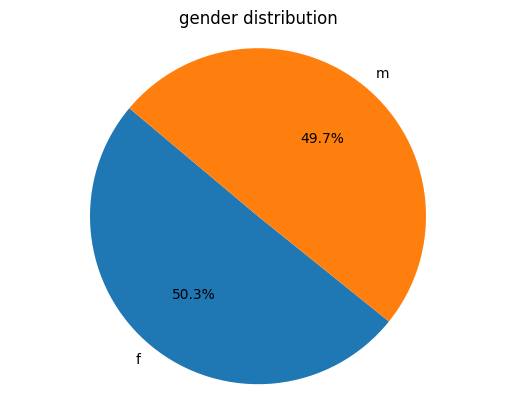
\includegraphics[width=0.8\textwidth]{assets/gender distribution.png}
    \caption{Gender Distribution in the Adience Benchmark Dataset}
\end{figure}



\subsection{Age Distribution Analysis}

After standardization, the age distribution across the eight defined ranges was:

\begin{itemize}
    \item (0, 2): 2,491 samples (13.4\%)
    \item (4, 6): 2,158 samples (11.6\%)
    \item (8, 12): 2,287 samples (12.3\%)
    \item (15, 20): 1,642 samples (8.9\%)
    \item (25, 32): 5,391 samples (29.1\%) 
    \item (38, 43): 2,695 samples (14.5\%)
    \item (48, 53): 990 samples (5.3\%)
    \item (60, 100): 896 samples (4.8\%) 
\end{itemize}

\begin{figure}[H]
    \centering
    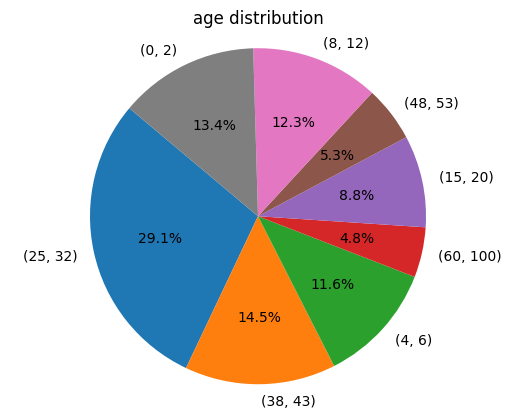
\includegraphics[width=0.8\textwidth]{assets/age distribution.png}
    \caption{Age Distribution in the Adience Benchmark Dataset}
\end{figure}


\subsection{Combined Age-Gender Analysis}

The intersection of age and gender categories revealed interesting patterns:

\begin{itemize}
    \item The (25, 32) age range showed the highest representation for both genders, with 3,026 female and 2,363 male samples.
    \item Gender distribution within age groups varied significantly:
    \begin{itemize}
        \item (0, 2): 684 female vs. 1,807 male 
        \item (8, 12): 1,353 female vs. 932 male
        \item (25, 32): 3,026 female vs. 2,363 male
        \item (48, 53): 458 female vs. 532 male
        \item (60, 100): 428 female vs. 467 male
    \end{itemize}
\end{itemize}

\paragraph{}
This combined analysis provides valuable insights into potential intersectional biases that might emerge during model training, particularly in the youngest age group where gender assignment was artificial rather than determined from image features.


\begin{figure}[H]
    \centering
    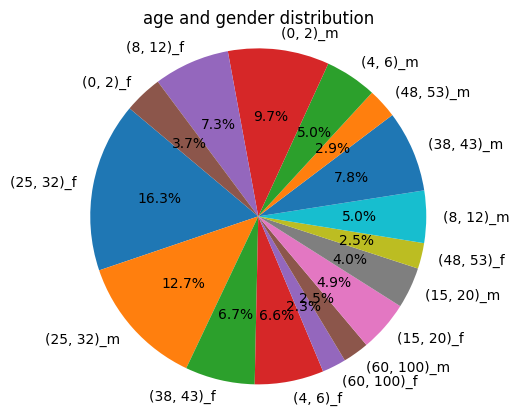
\includegraphics[width=0.8\textwidth]{assets/age and gender distribution.png}
    \caption{Combined Age and Gender Distribution in the Adience Benchmark Dataset}
\end{figure}

\subsection{Data Partitioning and Integrity}

To ensure proper evaluation methodology, we split the dataset into three partitions:

\begin{itemize}
    \item Training set: 11,850 samples (63.9\%)
    \item Validation set: 2,963 samples (16.0\%)
    \item Test set: 3,729 samples (20.1\%)
\end{itemize}

We rigorously verified that no overlap existed between these sets by checking the intersection between training and testing data based on image identifiers and face IDs. This verification confirmed complete separation, which is crucial for unbiased performance evaluation.

\section*{Tools used in the project}

The following tools and techniques were used in this project :

\begin{itemize}
    \item Softmax
    \item SVM
    \item Random Forest
    \item Adaboost
    \item KNN
    \item Multi-layer Perceptron (MLP)
    \item PCA 
    \item ResNet50- as feature extractor and as a model
\end{itemize}

\newpage
\section{Training Methodology}

\subsection{Feature Extraction}

For most of our models, we used pre-trained networks to extract meaningful features from face images rather than training directly on raw pixel values. This approach, known as transfer learning, leverages knowledge from models pre-trained on large datasets.

\begin{itemize}
    \item \textbf{ResNet50 Feature Extraction}: We utilized the ResNet50 architecture pre-trained on ImageNet to transform raw images into 2048-dimensional feature vectors. This was implemented for both RGB and grayscale processing pipelines.
    
    \item \textbf{Image Preprocessing}: Before feature extraction, images were resized to 224×224 pixels and normalized according to ImageNet statistics. For grayscale processing, single-channel images were duplicated across three channels to match ResNet50's input requirements.
    
    \item \textbf{Batch Processing}: To manage memory efficiently, images were processed in batches of 64, with separate feature sets created for training, validation, and test partitions.
\end{itemize}

We also try PCA as a feature extraction method, but the results were not as good as the ResNet50 feature extraction method, so we decided to use the ResNet50 feature extraction method for our models.

\subsection{Data Preprocessing}

After feature extraction, several preprocessing steps were applied to prepare the data for model training:

\begin{itemize}
    \item \textbf{Feature Standardization}: Features were standardized to have zero mean and unit variance using scikit-learn's StandardScaler, fitted on the training set and applied to both validation and test sets.
    
    \item \textbf{Label Encoding}: The combined age and gender labels (e.g., "(25, 32)\_f" for a female in the 25-32 age range) were encoded into numeric indices using LabelEncoder.
    
    \item \textbf{Class Weights}: To address class imbalance in the dataset, we computed balanced class weights inversely proportional to class frequencies, ensuring that minority classes received appropriate attention during training.
\end{itemize}

\subsection{Model Training Approaches}

We trained two parallel sets of models—one using RGB features and another using grayscale features—to compare their effectiveness:

\begin{itemize}
    \item \textbf{Traditional Machine Learning}: For Softmax (Logistic Regression), SVM, Random Forest, AdaBoost, and KNN models, we used scikit-learn implementations.
    
    \item \textbf{Neural Network Models}: For MLP model, we implemented architectures in TensorFlow with dropout and batch normalization to prevent overfitting. Training used the Adam optimizer with categorical cross-entropy loss and early stopping based on validation set performance.
    
    \item \textbf{CNN Training}: These models were trained directly on image data rather than on extracted features.
\end{itemize}

\subsection{Evaluation Methodology}

To ensure robust evaluation of model performance:

\begin{itemize}
    \item \textbf{Metrics}: We primarily used accuracy as our evaluation metric, calculated on both training and test sets to assess overfitting.
    
    \item \textbf{Confusion Matrix Analysis}: We analyzed confusion matrices to understand the types of errors made by each model, particularly focusing on whether errors occurred between adjacent age groups or across gender boundaries.
    
    \item \textbf{Cross-Comparison}: Performance was compared across RGB and grayscale processing pipelines to determine whether color information provided meaningful advantages.
\end{itemize}

All models were saved after training for later deployment and testing in real-world scenarios, which informed our analysis of practical applications detailed in the research questions section.

\newpage
\section{Model Performance}
\subsection{Grayscale scores}

\subsubsection{Grayscale Model Training and Testing Accuracy}
Table \ref{tab:Grayscale scores} summarizes the accuracy results of different models on the dataset using grayscale image.

\begin{table}[htbp]
    \centering
    \begin{tabular}{lccc}
        \toprule
        Model & Train Accuracy & Test Accuracy & Notes \\
        \toprule
        Softmax & 0.7095 & 0.3135 & \parbox[t]{6cm}{most of the error in the confusion matrix was in the adjacent age group.} \\
        \midrule
        SVM & 0.2046 & 0.1781 & \parbox[t]{6cm}{the model predict for the most of the data to 25-32 age group, and the gender was female.} \\
        \midrule
        Random Forest & 0.7730 & 0.3167 & \parbox[t]{6cm}{the model predict for the most of the data to 25-32 age group, but he got the gender right.} \\
        \midrule
        AdaBoost & 0.3467 & 0.2650 & \parbox[t]{6cm}{the  have berrly predict classes that he dont have a lot of data.} \\
        \midrule
        K-NN (k=1) & 0.9998 & 0.2202 & \parbox[t]{6cm}{we can see the overfitting -  the train accuracy is very high, but the test accuracy is very low.} \\
        \midrule
        K-NN (k=3) & 0.7525 & 0.2258 & \parbox[t]{6cm}{we can see start of overfitting - most of the error in the confusion matrix was near the (25,32) age group - the majority class.}\\
        \midrule
        K-NN (k=5) & 0.7001 & 0.2314 & \parbox[t]{6cm}{the over fitting is less significant}\\
        \midrule
        K-NN (k=7) & 0.6631 & 0.2422 & \parbox[t]{6cm}{the over fitting is less significant} \\
        \midrule
        K-NN (k=9) & 0.6331 & 0.2440 &  \parbox[t]{6cm}{the over fitting is less significant} \\
        \midrule
        MLP & 0.7521 & 0.3229 & \parbox[t]{6cm}{the model with the less overfitting, and when the model got wrong predictions, it was not by much (the most of the error in the confusion matrix was in the adjacent age group).} \\
        \midrule
        CNN & 0.4371 & 0.3153 & \parbox[t]{6cm}{this model have overffiting - it predict most of the data to the (25,32) age group.} \\
        \bottomrule
    \end{tabular}
    \caption{Train, Test, and Validation Accuracy of Various Models with grayscale method}
    \label{tab:Grayscale scores}
\end{table}

\subsubsection{Grayscale Model Confusion Matrices}

The following confusion matrices illustrate the classification patterns for each grayscale model, showing where models tend to make correct predictions (diagonal) versus misclassifications (off-diagonal).

\begin{figure}[H]
    \centering
    \begin{subfigure}[b]{0.48\textwidth}
        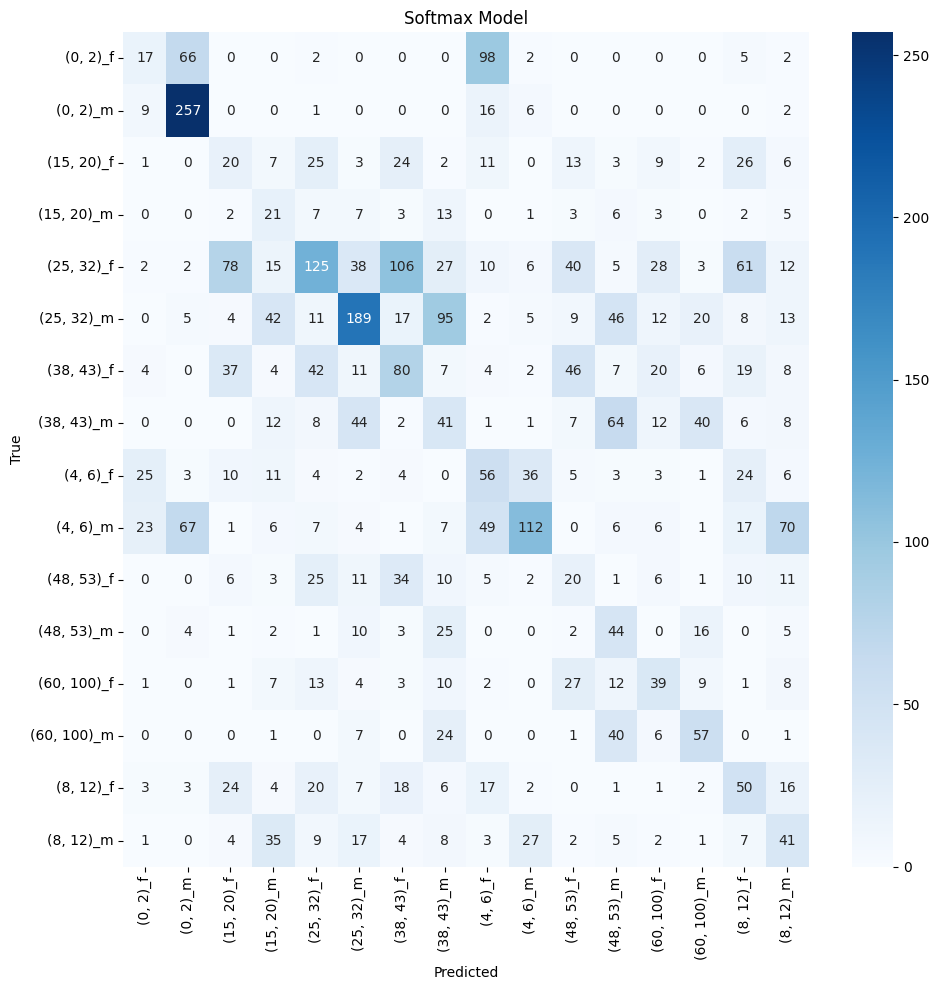
\includegraphics[width=\textwidth]{assets/confusion_matrix/grayscale/Softmax Model.png}
        \caption{Softmax}
    \end{subfigure}
    \hfill
    \begin{subfigure}[b]{0.48\textwidth}
        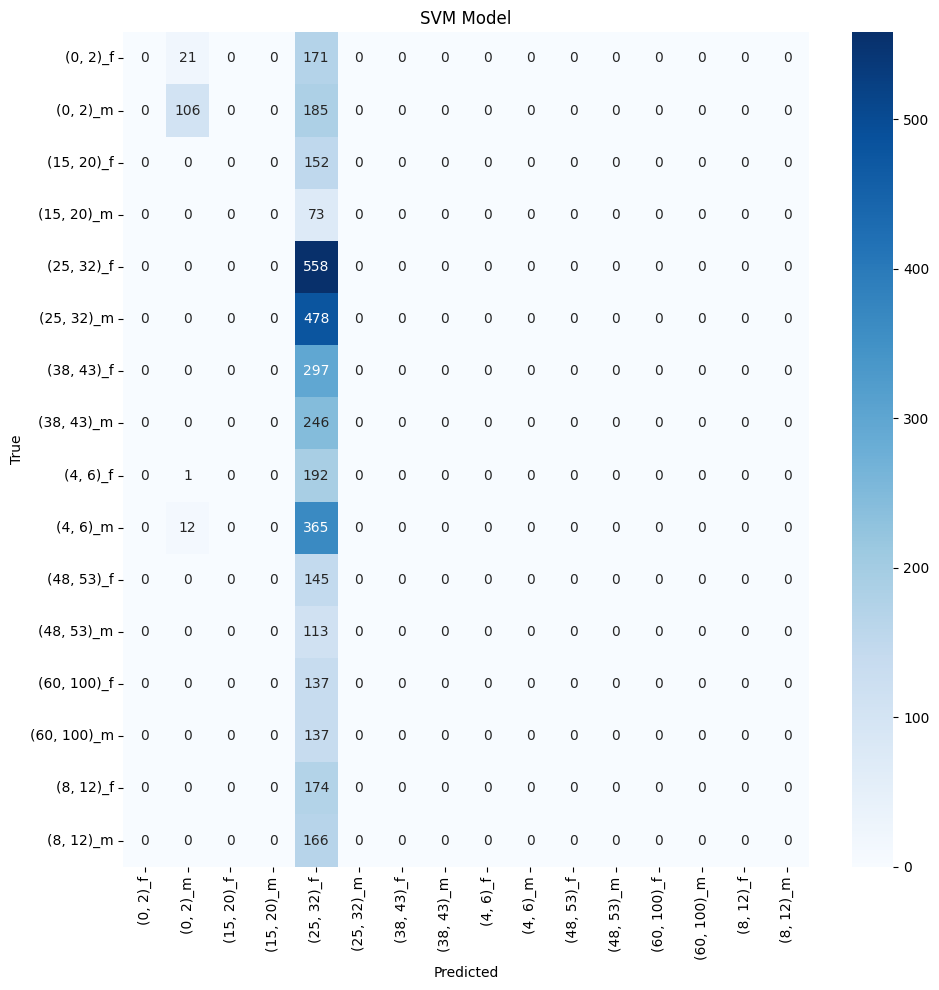
\includegraphics[width=\textwidth]{assets/confusion_matrix/grayscale/SVM Model.png}
        \caption{SVM}
    \end{subfigure}
    \caption{Confusion matrices for Softmax and SVM models (grayscale)}
    \label{fig:grayscale_confusion_matrices_1}
\end{figure}

\begin{figure}[H]
    \centering
    \begin{subfigure}[b]{0.48\textwidth}
        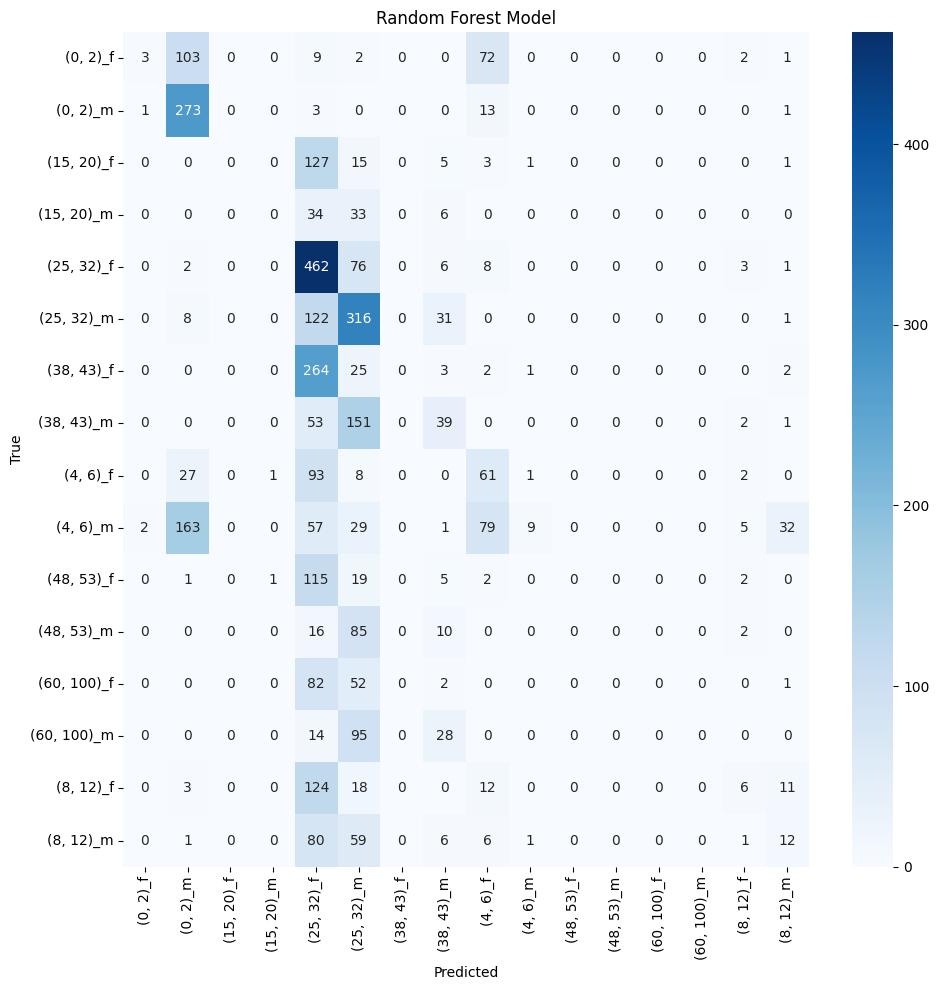
\includegraphics[width=\textwidth]{assets/confusion_matrix/grayscale/RF Model.png}
        \caption{Random Forest}
    \end{subfigure}
    \hfill
    \begin{subfigure}[b]{0.48\textwidth}
        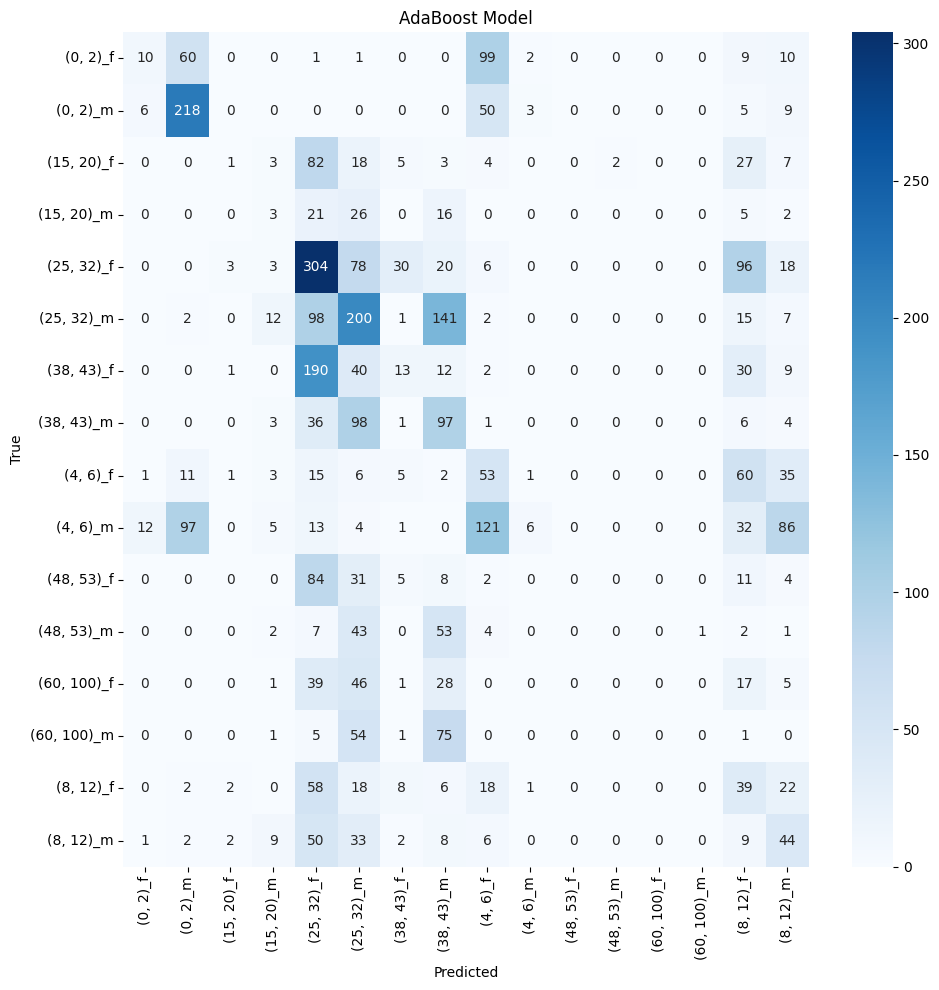
\includegraphics[width=\textwidth]{assets/confusion_matrix/grayscale/AdaBoost Model.png}
        \caption{AdaBoost}
    \end{subfigure}
    \caption{Confusion matrices for Random Forest and AdaBoost models (grayscale)}
    \label{fig:grayscale_confusion_matrices_2}
\end{figure}

\begin{figure}[H]
    \centering
    \begin{subfigure}[b]{0.48\textwidth}
        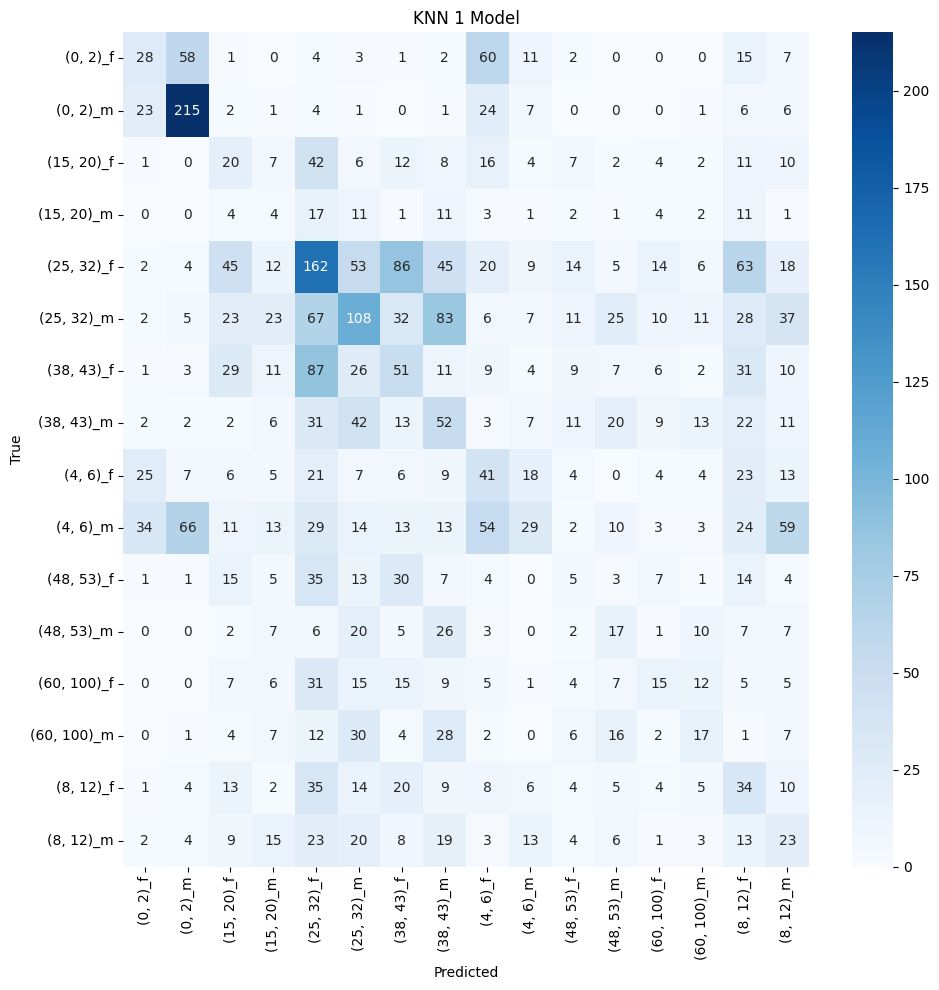
\includegraphics[width=\textwidth]{assets/confusion_matrix/grayscale/KNN1.png}
        \caption{KNN (k=1)}
    \end{subfigure}
    \hfill
    \begin{subfigure}[b]{0.48\textwidth}
        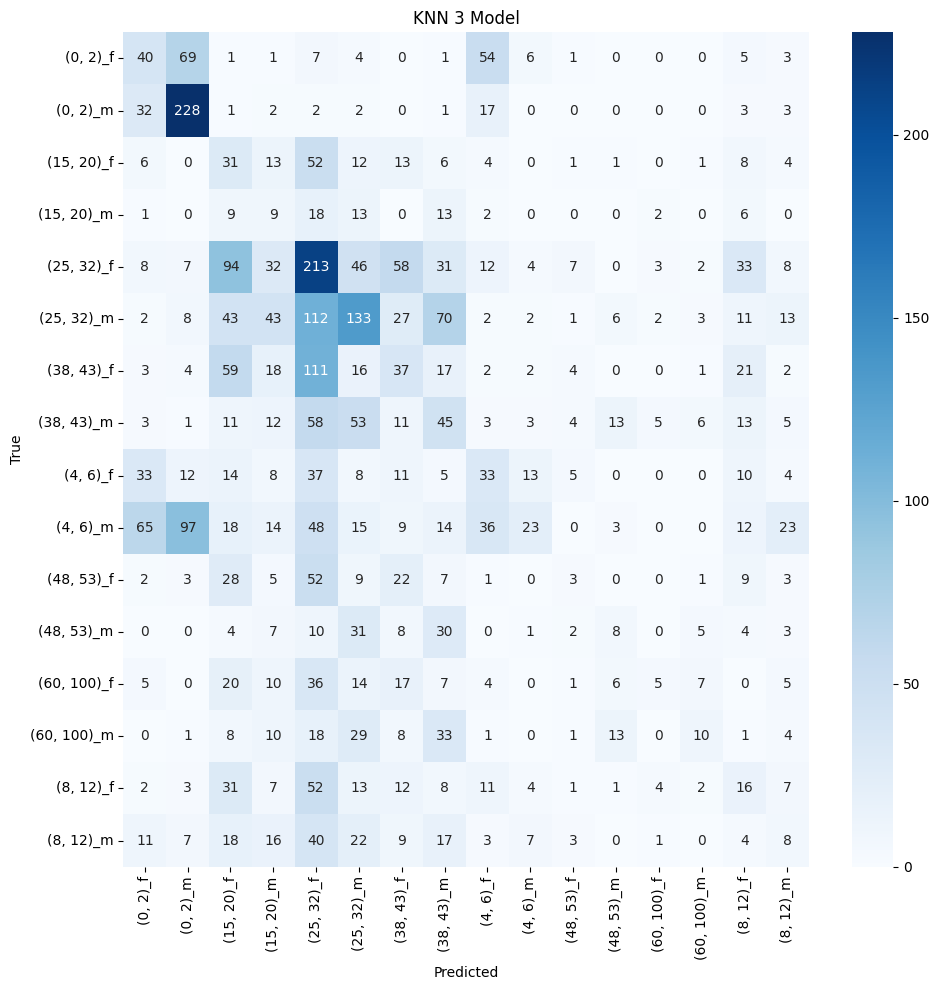
\includegraphics[width=\textwidth]{assets/confusion_matrix/grayscale/KNN3.png}
        \caption{KNN (k=3)}
    \end{subfigure}
    \caption{Confusion matrices for KNN models with k=1 and k=3 (grayscale)}
    \label{fig:grayscale_confusion_matrices_3}
\end{figure}

\begin{figure}[H]
    \centering
    \begin{subfigure}[b]{0.48\textwidth}
        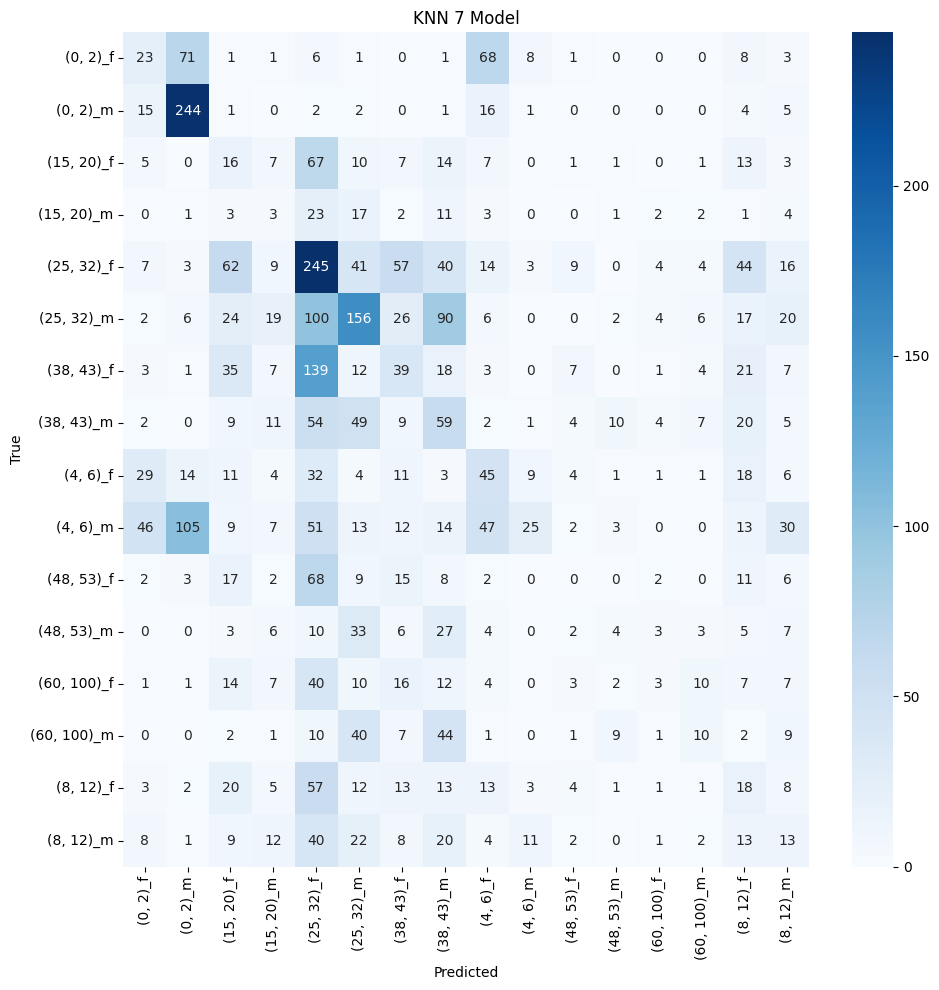
\includegraphics[width=\textwidth]{assets/confusion_matrix/grayscale/KNN7.png}
        \caption{KNN (k=7)}
    \end{subfigure}
    \hfill
    \begin{subfigure}[b]{0.48\textwidth}
        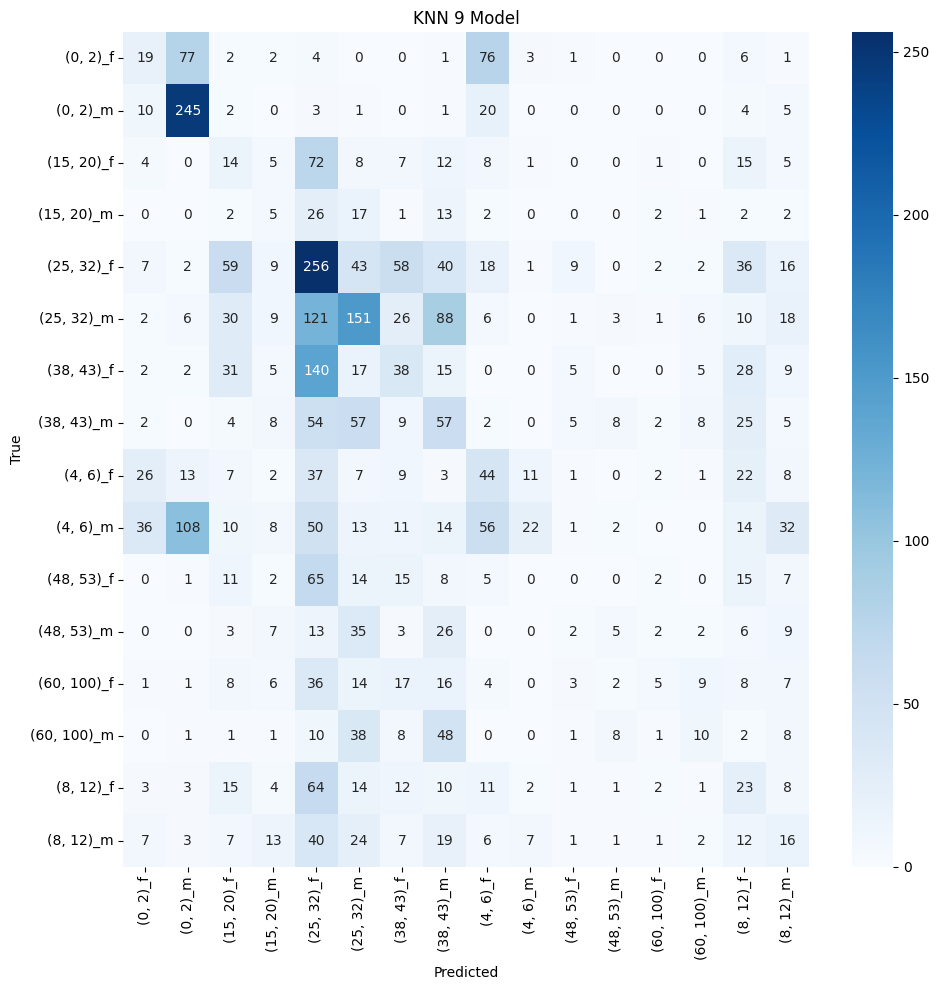
\includegraphics[width=\textwidth]{assets/confusion_matrix/grayscale/KNN9.png}
        \caption{KNN (k=9)}
    \end{subfigure}
    \caption{Confusion matrices for KNN models with k=7 and k=9 (grayscale)}
    \label{fig:grayscale_confusion_matrices_4}
\end{figure}

\begin{figure}[H]
    \centering
    \begin{subfigure}[b]{0.48\textwidth}
        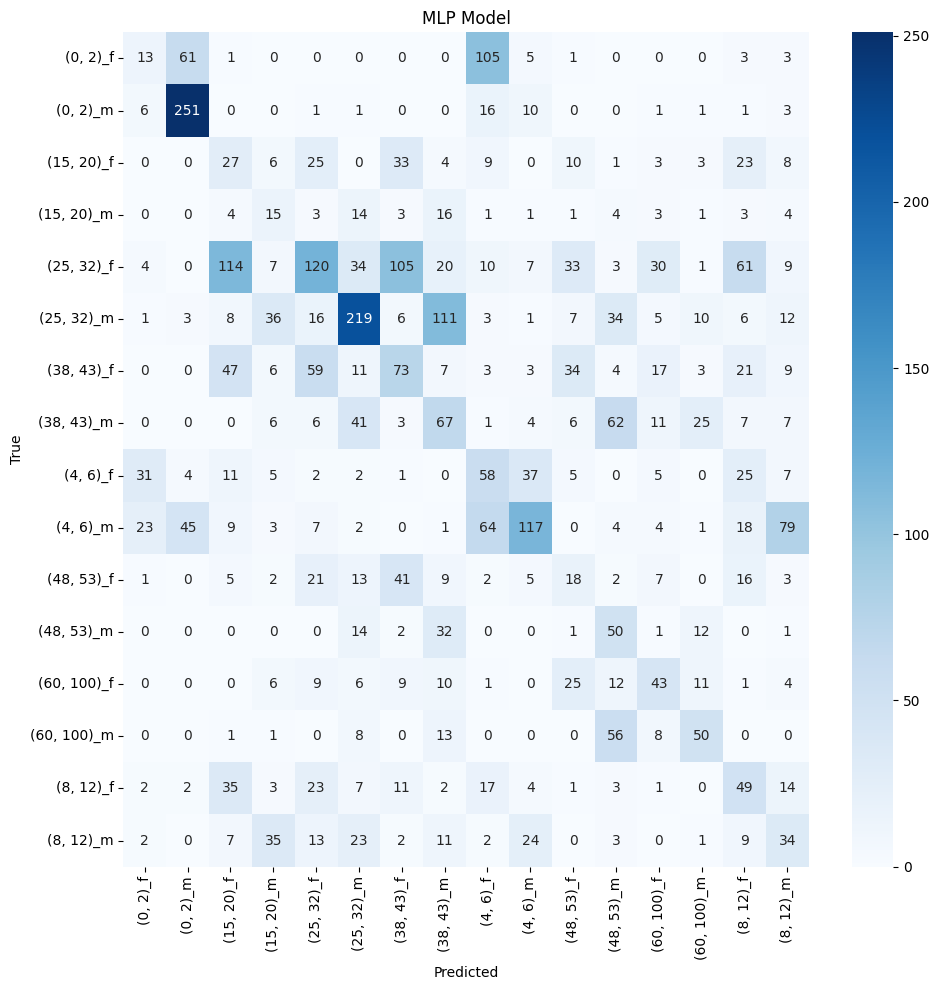
\includegraphics[width=\textwidth]{assets/confusion_matrix/grayscale/MLP.png}
        \caption{MLP}
    \end{subfigure}
    \hfill
    \begin{subfigure}[b]{0.48\textwidth}
        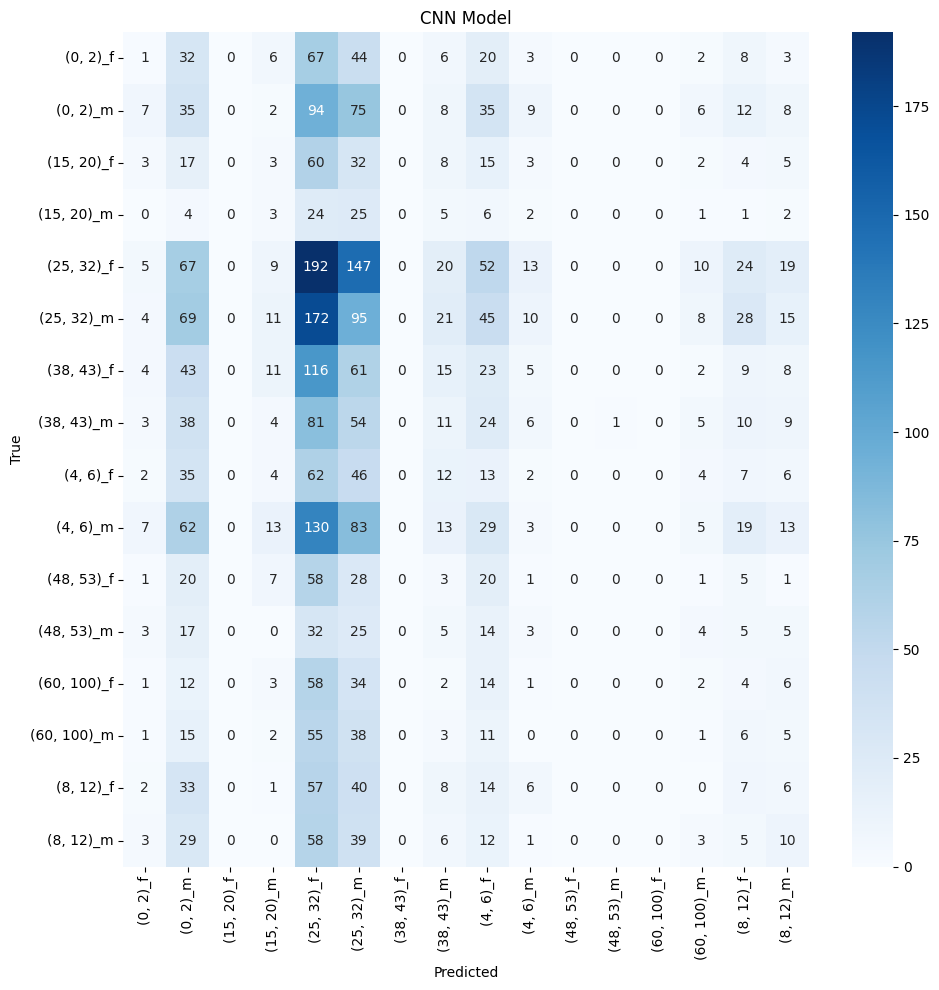
\includegraphics[width=\textwidth]{assets/confusion_matrix/grayscale/CNN.png}
        \caption{CNN}
    \end{subfigure}
    \caption{Confusion matrices for MLP and CNN models (grayscale)}
    \label{fig:grayscale_confusion_matrices_5}
\end{figure}

\begin{figure}[H]
    \centering
    \begin{subfigure}[b]{0.48\textwidth}
        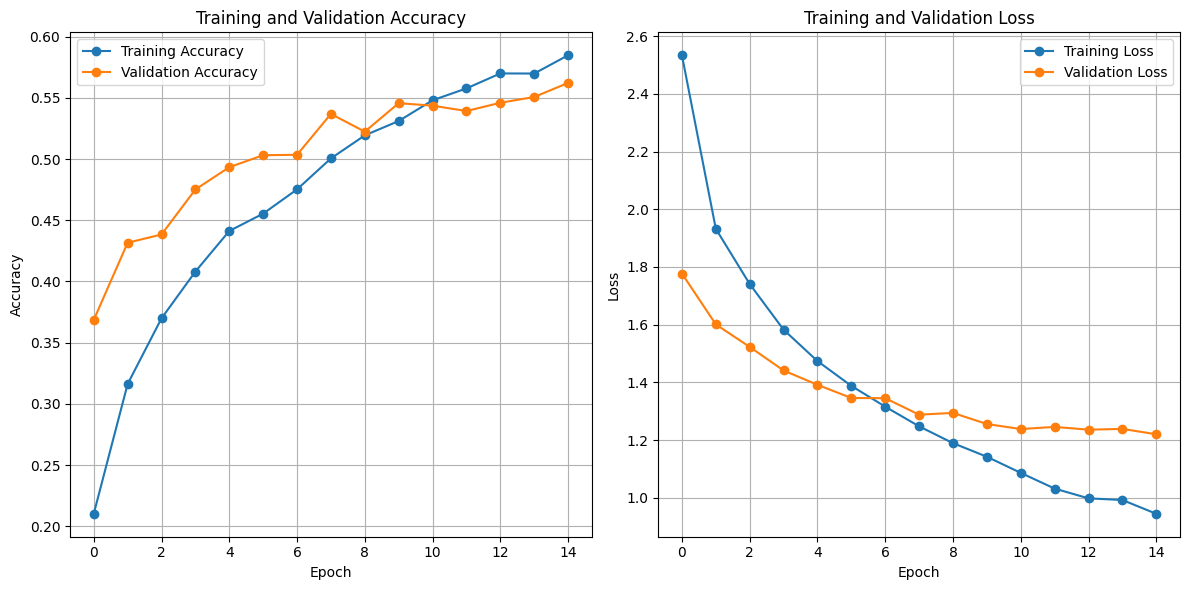
\includegraphics[width=\textwidth]{assets/confusion_matrix/grayscale/MLP_history.png}
        \caption{MLP training history}
    \end{subfigure}
    \hfill
    \begin{subfigure}[b]{0.48\textwidth}
        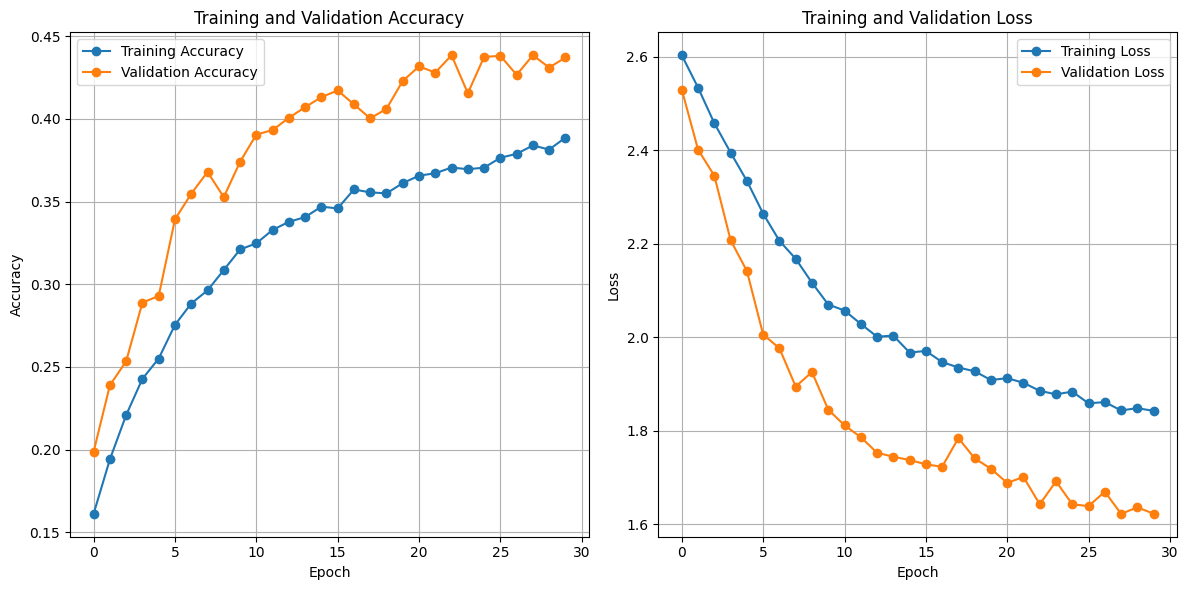
\includegraphics[width=\textwidth]{assets/confusion_matrix/grayscale/CNN_history.png}
        \caption{CNN training history}
    \end{subfigure}
    \caption{Taining history for MLP and CNN models (grayscale)}
    \label{fig:grayscale_training_history}
\end{figure}


\FloatBarrier 
\newpage
\subsection{RGB scores}
\subsubsection{RGB Model Training and Testing Accuracy}
Table \ref{tab:RGB scores} summarizes the accuracy results of different models on the dataset using RGB image. (we dont add a Note column because the results are similar to the grayscale image)

\begin{table}[htbp] % Allow flexibility in positioning
    \centering
    \begin{tabular}{lcc}
        \toprule
        Model & Train Accuracy & Test Accuracy \\
        \toprule
        Softmax & 0.7331 & 0.3237 \\
        \midrule
        SVM & 0.2045 & 0.1751 \\
        \midrule
        Random Forest & 0.7728 & 0.3218 \\
        \midrule
        AdaBoost & 0.3716 & 0.3162 \\
        \midrule
        K-NN (k=1) & 0.9998 & 0.1917 \\
        \midrule
        K-NN (k=3) & 0.7778 & 0.2092 \\
        \midrule
        K-NN (k=7) & 0.6886 & 0.2279 \\
        \midrule
        K-NN (k=9) & 0.6658 & 0.2333 \\
        \midrule
        MLP & 0.7950 & 0.3478 \\
        \midrule
        CNN & 0.4718 & 0.3298 \\
        \bottomrule
    \end{tabular}
    \caption{Train and Test Accuracy of Various Models with RGB image}
    \label{tab:RGB scores}
\end{table}
\FloatBarrier 

\subsubsection{RGB Model Confusion Matrices}

The following confusion matrices illustrate the classification patterns for each rgb model, showing where models tend to make correct predictions (diagonal) versus misclassifications (off-diagonal).

\begin{figure}[H]
    \centering
    \begin{subfigure}[b]{0.48\textwidth}
        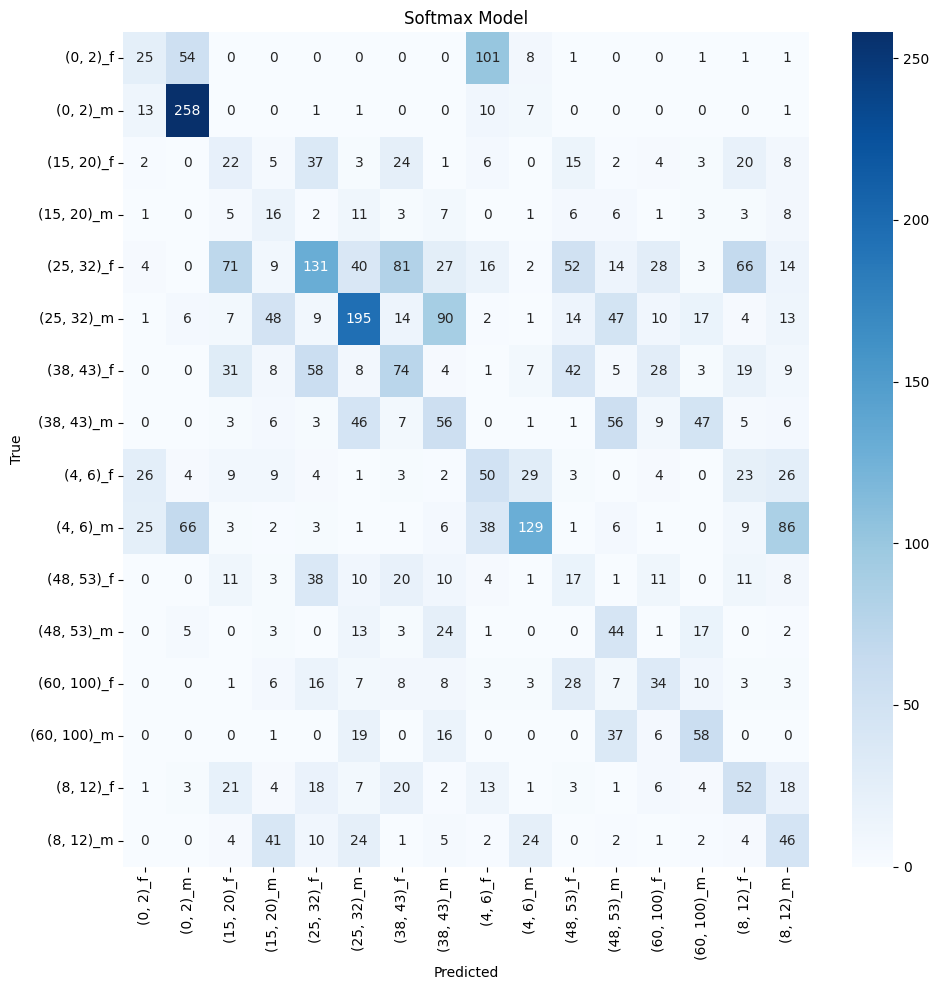
\includegraphics[width=\textwidth]{assets/confusion_matrix/rgb/Softmax Model.png}
        \caption{Softmax}
    \end{subfigure}
    \hfill
    \begin{subfigure}[b]{0.48\textwidth}
        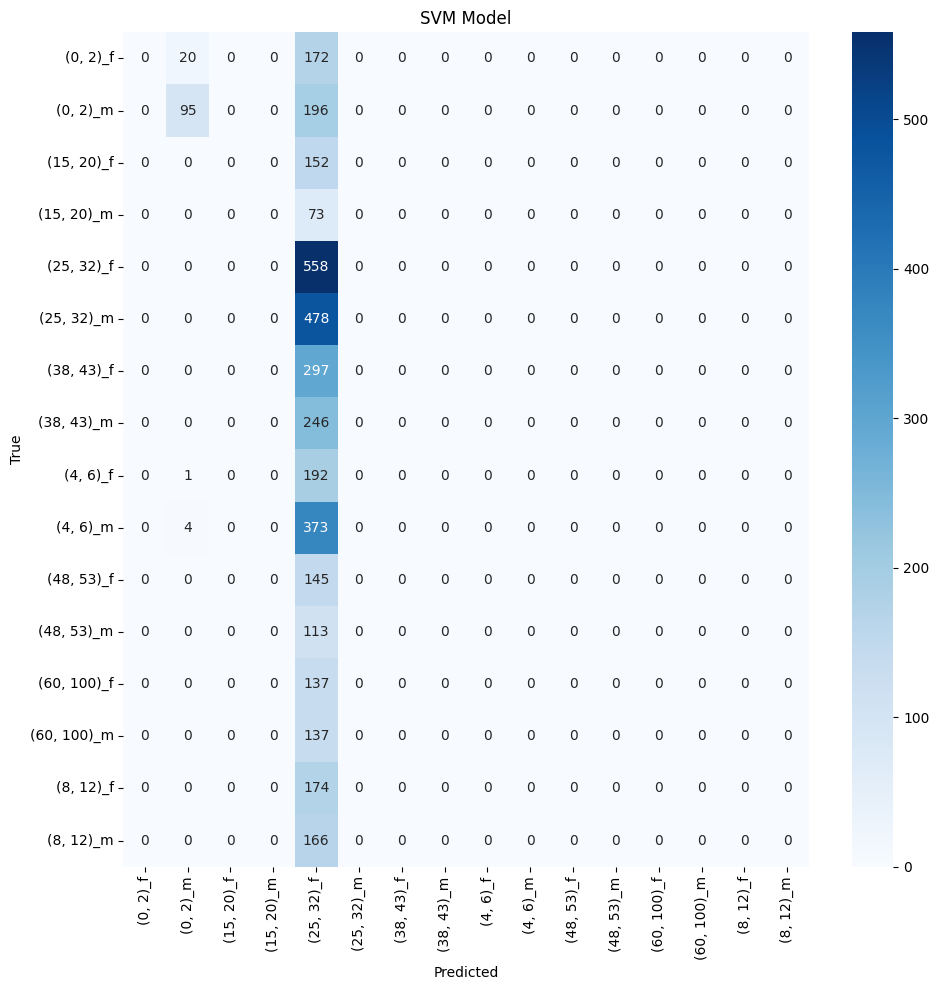
\includegraphics[width=\textwidth]{assets/confusion_matrix/rgb/SVM Model.png}
        \caption{SVM}
    \end{subfigure}
    \caption{Confusion matrices for Softmax and SVM models (rgb)}
    \label{fig:rgb_confusion_matrices_1}
\end{figure}

\begin{figure}[H]
    \centering
    \begin{subfigure}[b]{0.48\textwidth}
        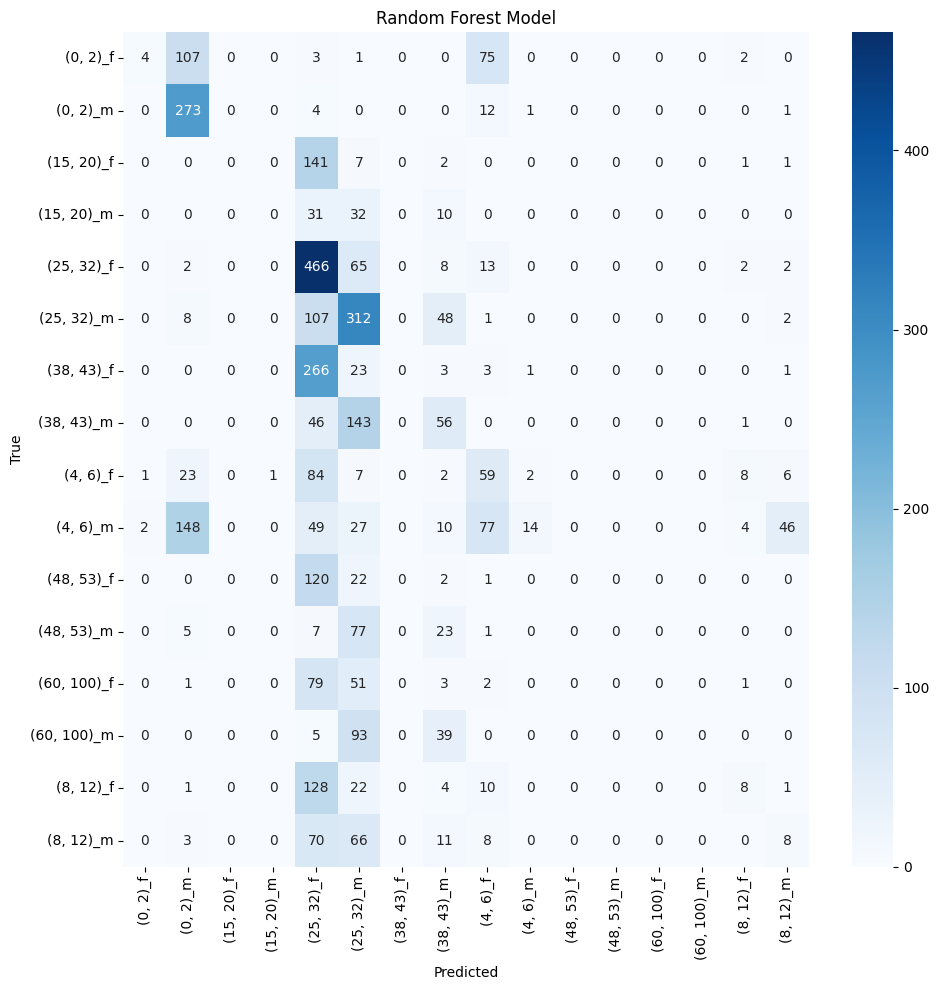
\includegraphics[width=\textwidth]{assets/confusion_matrix/rgb/RF Model.png}
        \caption{Random Forest}
    \end{subfigure}
    \hfill
    \begin{subfigure}[b]{0.48\textwidth}
        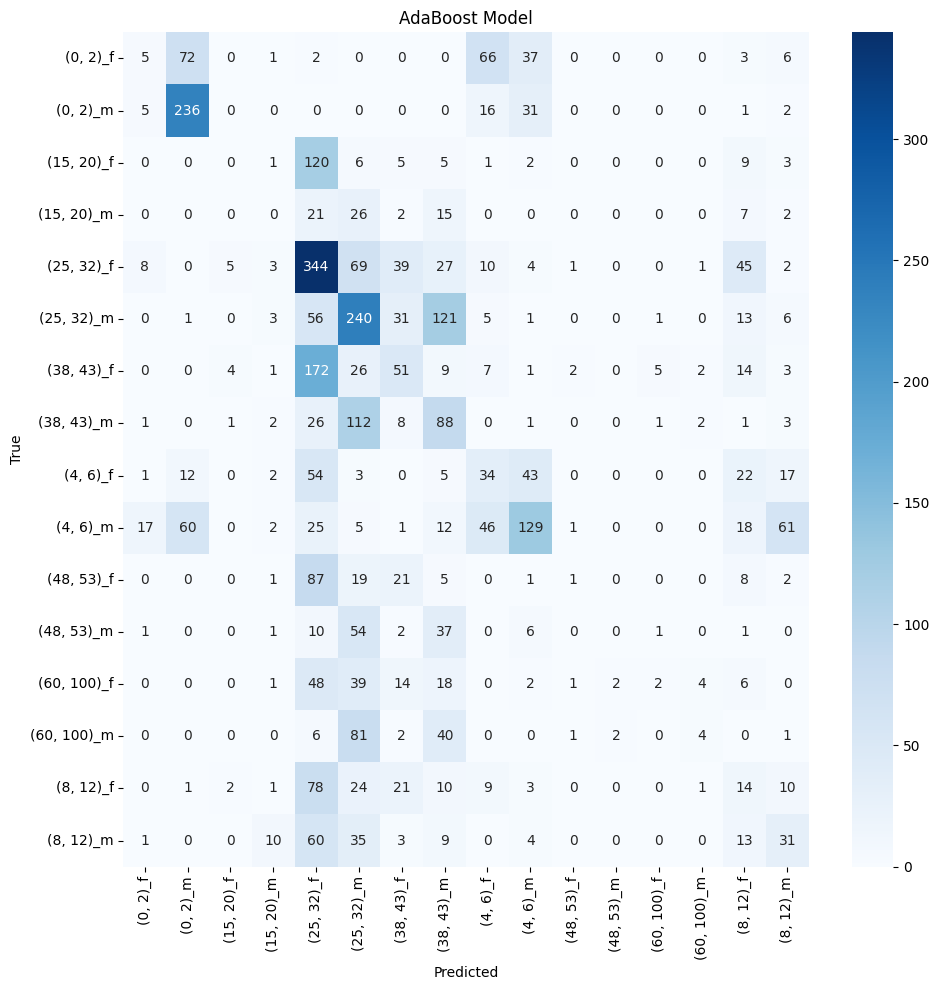
\includegraphics[width=\textwidth]{assets/confusion_matrix/rgb/AdaBoost Model.png}
        \caption{AdaBoost}
    \end{subfigure}
    \caption{Confusion matrices for Random Forest and AdaBoost models (rgb)}
    \label{fig:rgb_confusion_matrices_2}
\end{figure}

\begin{figure}[H]
    \centering
    \begin{subfigure}[b]{0.48\textwidth}
        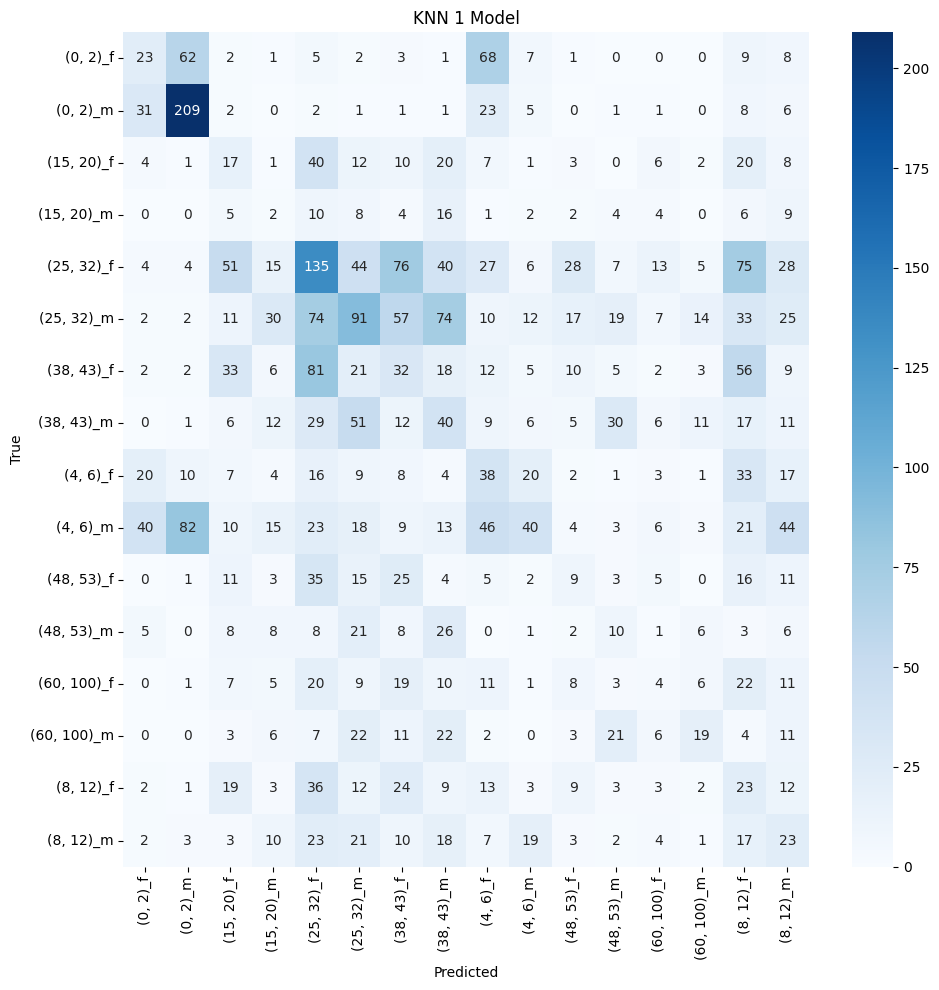
\includegraphics[width=\textwidth]{assets/confusion_matrix/rgb/KNN1.png}
        \caption{KNN (k=1)}
    \end{subfigure}
    \hfill
    \begin{subfigure}[b]{0.48\textwidth}
        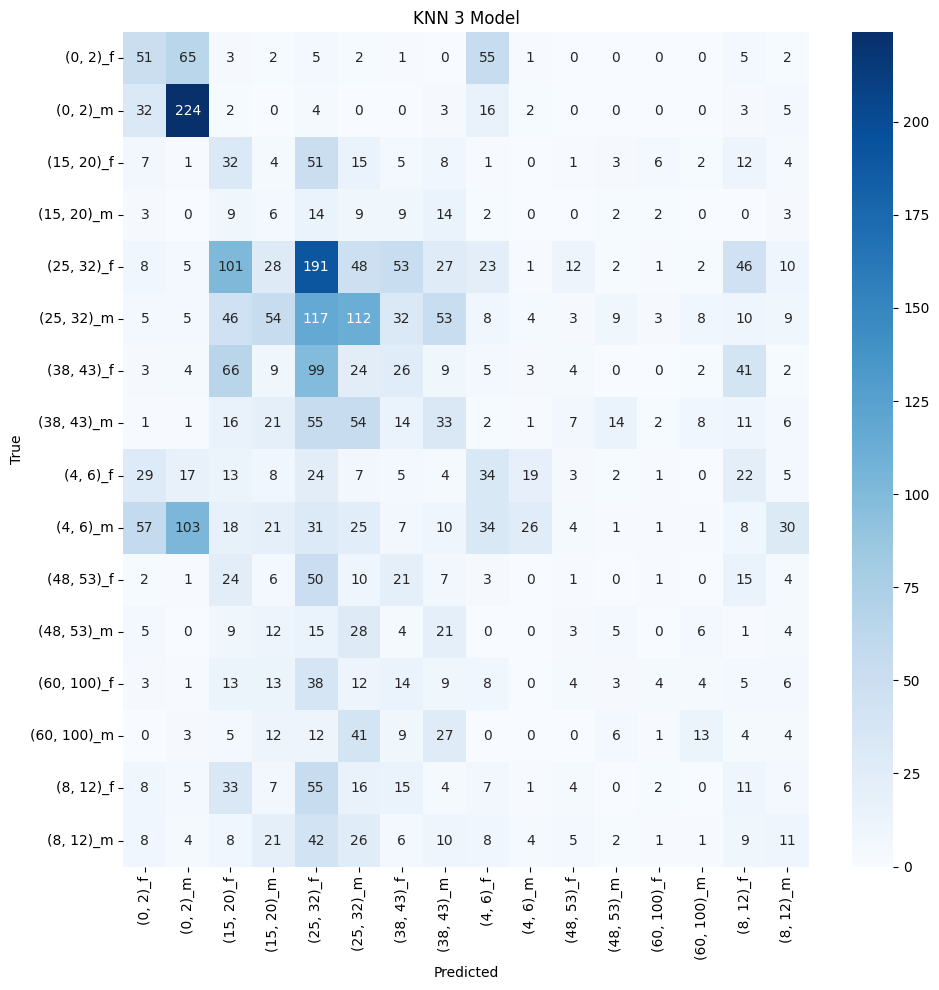
\includegraphics[width=\textwidth]{assets/confusion_matrix/rgb/KNN3.png}
        \caption{KNN (k=3)}
    \end{subfigure}
    \caption{Confusion matrices for KNN models with k=1 and k=3 (rgb)}
    \label{fig:rgb_confusion_matrices_3}
\end{figure}

\begin{figure}[H]
    \centering
    \begin{subfigure}[b]{0.48\textwidth}
        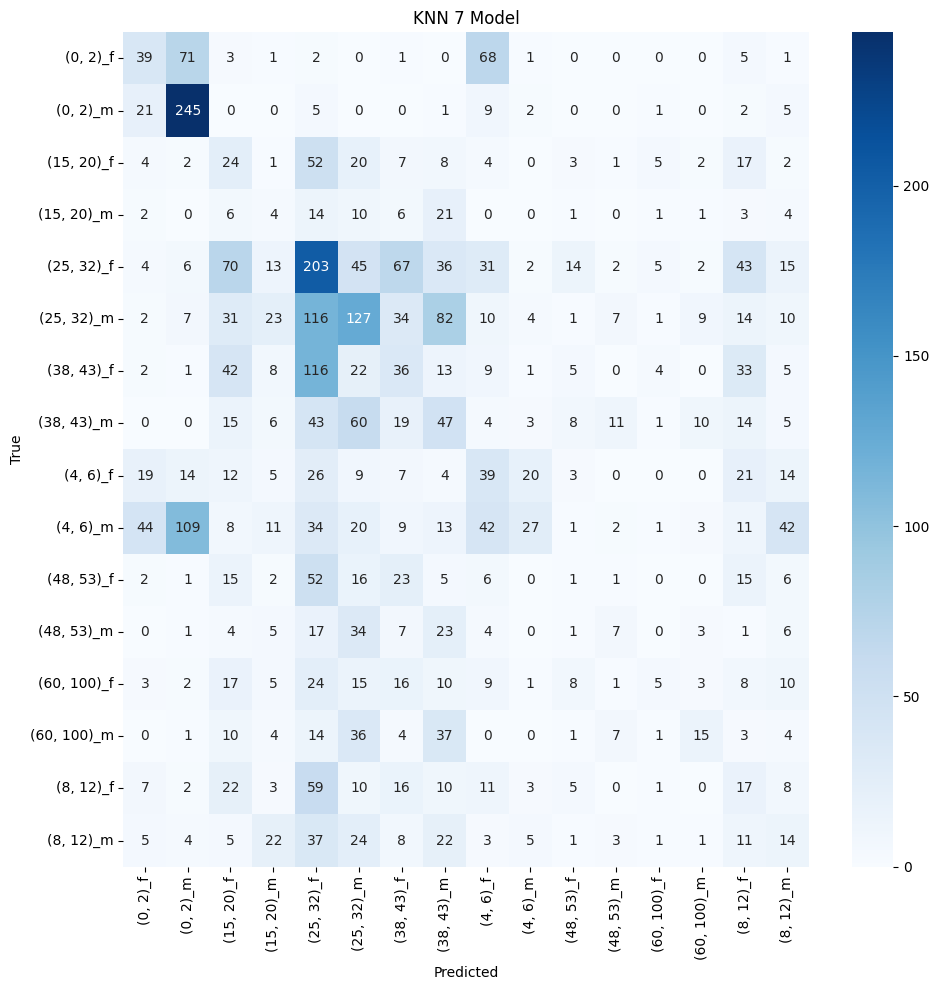
\includegraphics[width=\textwidth]{assets/confusion_matrix/rgb/KNN7.png}
        \caption{KNN (k=7)}
    \end{subfigure}
    \hfill
    \begin{subfigure}[b]{0.48\textwidth}
        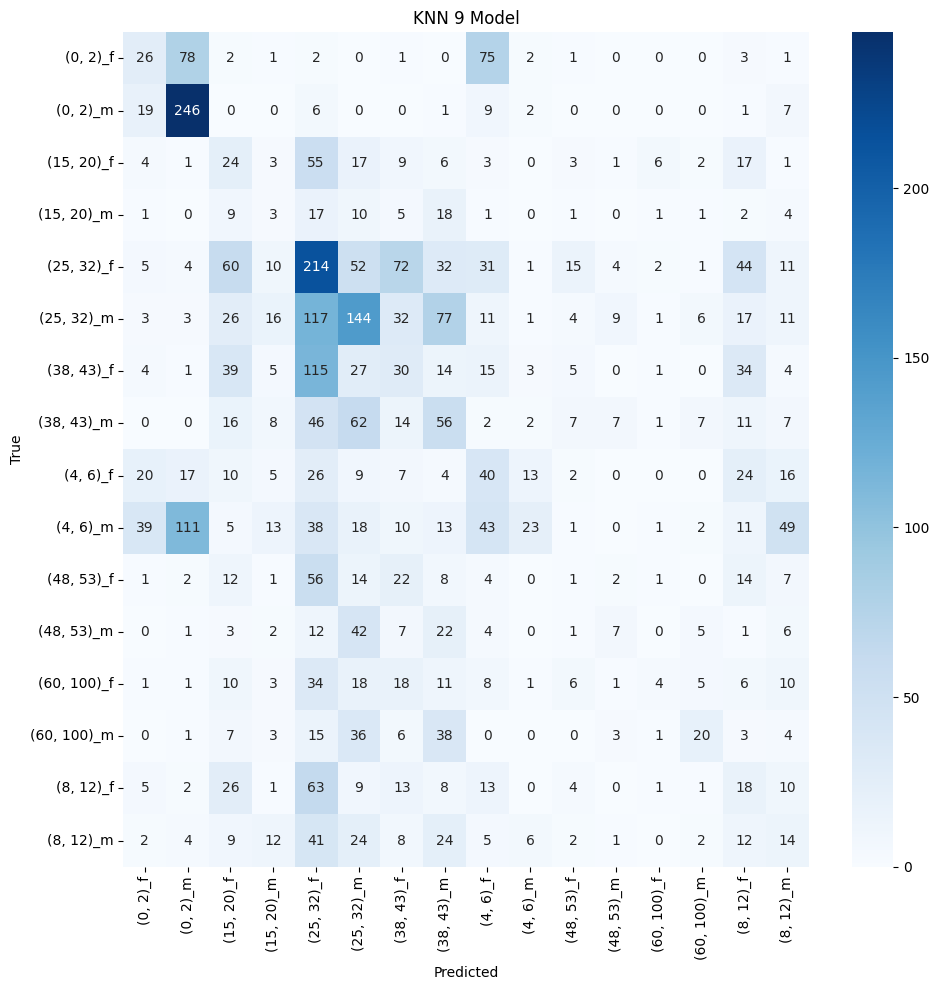
\includegraphics[width=\textwidth]{assets/confusion_matrix/rgb/KNN9.png}
        \caption{KNN (k=9)}
    \end{subfigure}
    \caption{Confusion matrices for KNN models with k=7 and k=9 (rgb)}
    \label{fig:rgb_confusion_matrices_4}
\end{figure}

\begin{figure}[H]
    \centering
    \begin{subfigure}[b]{0.48\textwidth}
        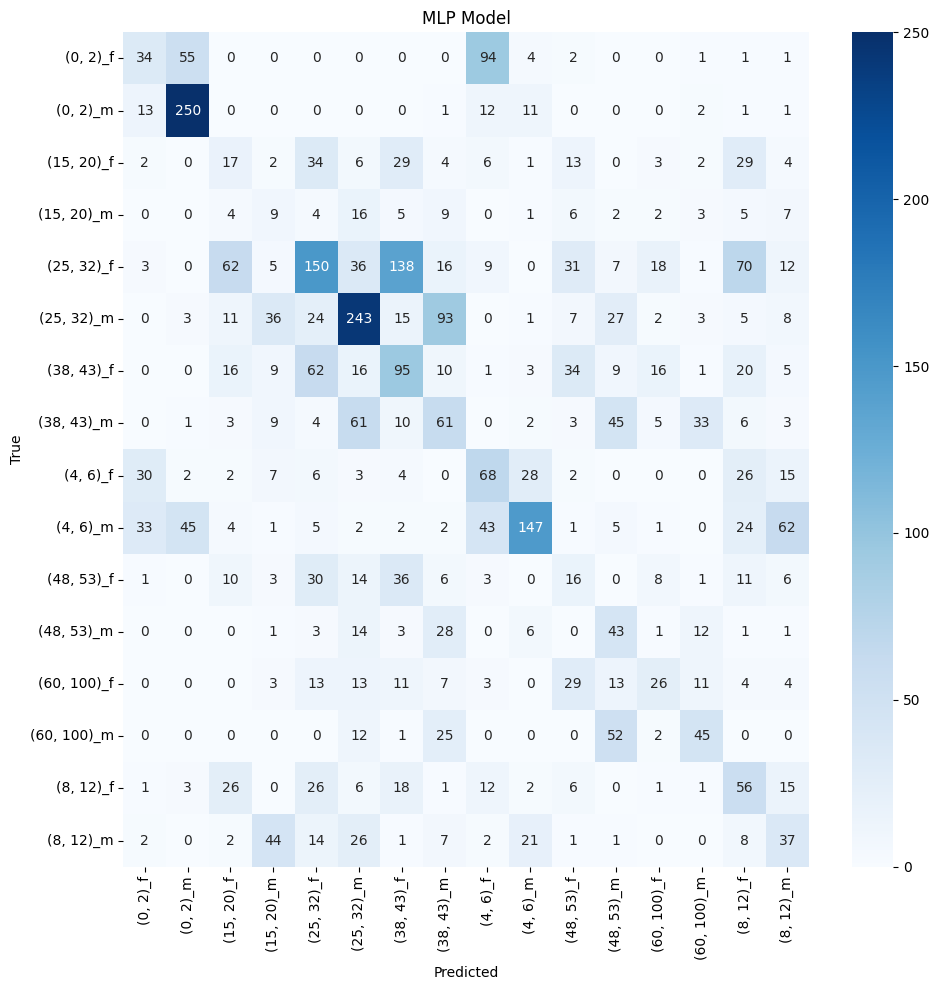
\includegraphics[width=\textwidth]{assets/confusion_matrix/rgb/MLP.png}
        \caption{MLP}
    \end{subfigure}
    \hfill
    \begin{subfigure}[b]{0.48\textwidth}
        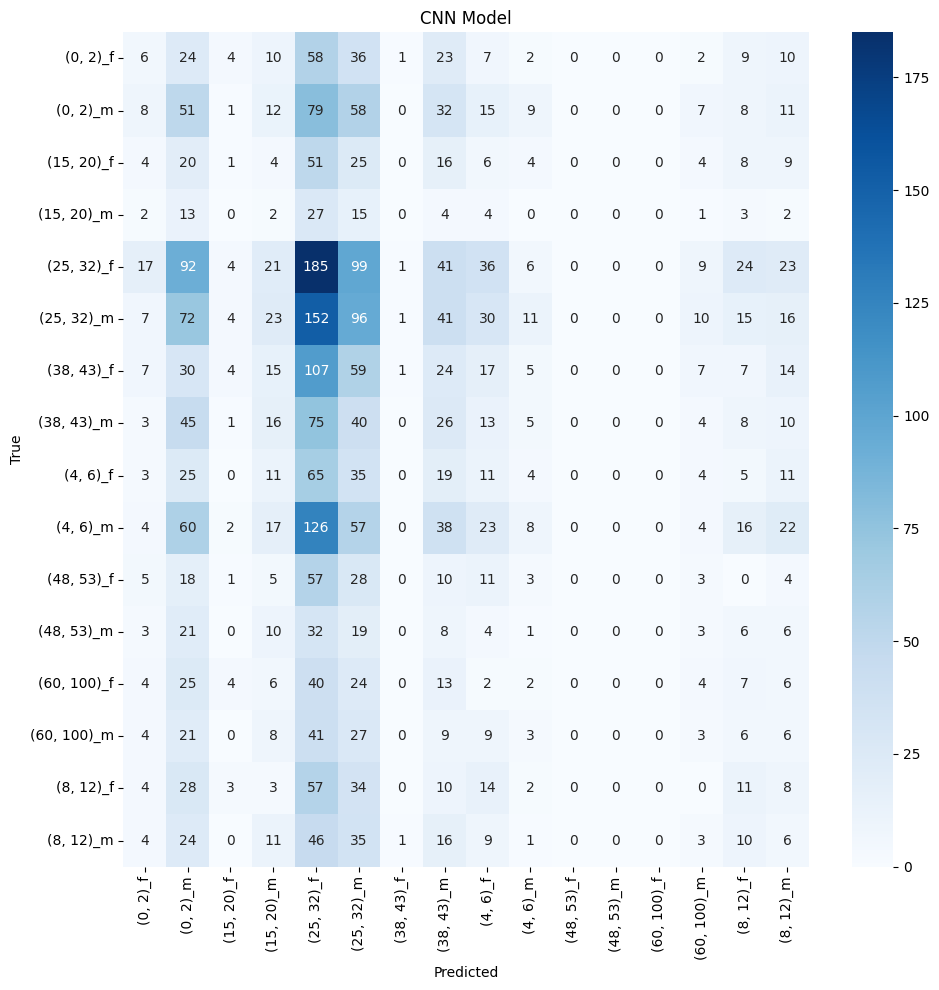
\includegraphics[width=\textwidth]{assets/confusion_matrix/rgb/CNN.png}
        \caption{CNN}
    \end{subfigure}
    \caption{Confusion matrices for MLP and CNN models (rgb)}
    \label{fig:rgb_confusion_matrices_5}
\end{figure}

\begin{figure}[H]
    \centering
    \begin{subfigure}[b]{0.48\textwidth}
        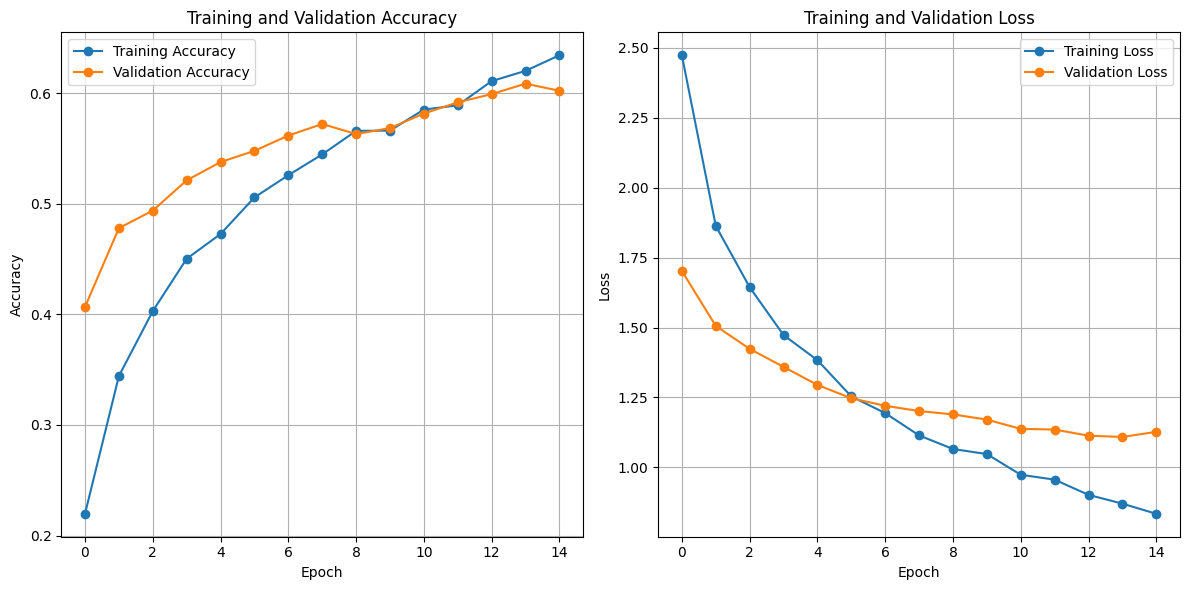
\includegraphics[width=\textwidth]{assets/confusion_matrix/rgb/MLP_history.png}
        \caption{MLP training history}
    \end{subfigure}
    \hfill
    \begin{subfigure}[b]{0.48\textwidth}
        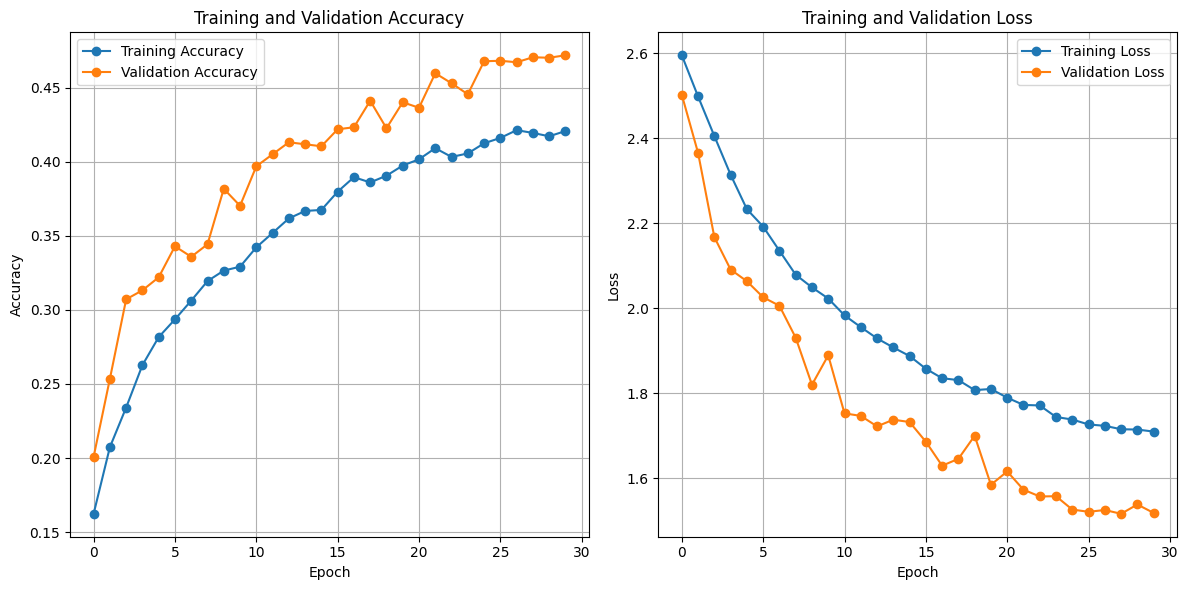
\includegraphics[width=\textwidth]{assets/confusion_matrix/rgb/CNN_history.png}
        \caption{CNN training history}
    \end{subfigure}
    \caption{Taining history for MLP and CNN models (rgb)}
    \label{fig:rgb_training_history}
\end{figure}

\newpage
\subsection{Analysis of Results}

Our experimental results reveal several important patterns across different model architectures and input processing methods. This section provides a detailed analysis of these findings.

\subsubsection{General Performance Trends}

Overall, models trained on RGB features slightly outperformed their grayscale counterparts, suggesting that color information provides valuable signals for age and gender classification. The best-performing model was the MLP with RGB features (34.78\% test accuracy), while the poorest performer was the SVM (17.51\% test accuracy on RGB features).

The relatively modest test accuracies (17.51\% to 34.78\%) reflect the inherent difficulty of the 16-class joint age-gender classification task. For context, random guessing would yield approximately 6.25\% accuracy, so our models provide 3-5 times better performance than chance.

\subsubsection{Model-Specific Analysis}

\paragraph{Softmax Regression:} 
Softmax achieved reasonable performance (32.37\% test accuracy with RGB features) despite being one of the simplest models. This suggests that the decision boundaries in our feature space have some linear separability. The model's confusion matrix showed it performed best on majority classes like (0, 2)\_m and (25, 32)\_m, with most errors occurring between adjacent age groups rather than gender misclassification.

\paragraph{Support Vector Machine (SVM):}
SVM performed notably poorly (17.51\% test accuracy), suggesting that the complex, high-dimensional feature space was not amenable to the approach of finding optimal hyperplanes. The SVM predominantly predicted the (25, 32)\_f class—the most common in our dataset—indicating a strong bias toward majority classes despite our class weighting efforts.

\paragraph{Random Forest:}
Random Forest models performed well (32.18\% test accuracy with RGB), showing their ability to capture complex patterns through ensemble decision trees. The model effectively learned the feature importance patterns from ResNet50 embeddings, with depth-limited trees (max\_depth=10) helping to control overfitting. However, like most models, it struggled with underrepresented classes.

\paragraph{AdaBoost:}
AdaBoost showed moderate performance (31.62\% with RGB), focusing its learning on difficult-to-classify examples. This approach was particularly effective for our dataset with imbalanced classes, as evidenced by its relatively smaller gap between training and test accuracy compared to Random Forest.

\paragraph{K-Nearest Neighbors (KNN):}
KNN demonstrated clear patterns of overfitting, especially at lower k values. With k=1, the model achieved near-perfect training accuracy (99.98\%) but poor test performance (19.17\%), exemplifying "memorization" rather than generalization. As k increased, both overfitting and overall accuracy decreased, with k=9 showing the best test performance among KNN models. This confirms that allowing more neighbors to vote helps smooth decision boundaries in high-dimensional spaces.

\paragraph{Multi-Layer Perceptron (MLP):}
The MLP achieved the best overall performance (34.78\% test accuracy with RGB), demonstrating the advantage of deep learning architectures in capturing complex patterns. The network's combination of dense layers with dropout (0.5) and batch normalization effectively controlled overfitting while maintaining representational power. Early stopping further enhanced generalization by preventing overtraining.

\paragraph{Convolutional Neural Network (CNN):}
The CNN performed well (32.98\% with RGB) despite being trained directly on raw image data rather than pre-extracted features. This indicates that end-to-end learning can match transfer learning approaches on this task. However, the narrower gap between training (47.18\%) and testing (32.98\%) accuracy suggests that CNN architecture inherently provides some regularization compared to other models.

\subsubsection{Overfitting Analysis}

All models exhibited some degree of overfitting, visible in the gap between training and test accuracy. This can be attributed to several factors:

\begin{itemize}
    \item \textbf{Limited data diversity:} Despite having thousands of images, the number of samples per class was insufficient for reliable generalization across all 16 classes.
    
    \item \textbf{Class imbalance:} The uneven distribution of samples across age and gender categories made it difficult for models to learn accurate representations of minority classes.
    
    \item \textbf{High-dimensional feature space:} The 2048-dimensional ResNet50 features created a vast feature space relative to the number of training examples, making overfitting more likely.
\end{itemize}

\subsubsection{RGB vs. Grayscale Performance}

RGB models consistently outperformed their grayscale counterparts, though the margin was modest (typically 1-3 percentage points). This suggests that color information provides useful but not essential signals for age-gender classification. The color information may help with subtle cues like skin tone variations associated with aging or cosmetic differences between genders.

\subsubsection{Error Pattern Analysis}

Confusion matrices revealed consistent error patterns across models:

\begin{itemize}
    \item Most misclassifications occurred between adjacent age groups (e.g., (25, 32) and (38, 43)), highlighting the difficulty in precisely categorizing ages into distinct groups based on visual features alone.
    
    \item Gender misclassification was less common than age group errors, indicating that gender features are more distinct than age features in facial images.
    
    \item Certain age-gender combinations, particularly those with fewer training examples, showed consistently poorer classification results across all models.
\end{itemize}

This analysis suggests that while current models provide valuable age-gender classification capabilities, there remains significant room for improvement through more sophisticated architectures, data augmentation, and training strategies tailored to address the specific challenges of this multi-class classification problem.





\newpage
\section{Research Questions}

\subsection*{Question 1: How Models Work with Different Images}
\begin{itemize}[leftmargin=1.6cm]
    \item What happens when images are not clear or blurry?
    \item Do facial expressions (such as smiling or not smiling) affect the results?
\end{itemize}

\subsection*{Answer Question 1}
To investigate the impact of facial expressions on the predictions of the model,
we examined four different emotional states: smiling, serious, mad and regular. 
Our analysis revealed that all models produced consistent predictions in these expressions,
indicating that facial expressions do not significantly influence the results.


\subsection*{Question 2: Can We Use This in Real Life?}
\begin{itemize}[leftmargin=1.6cm]
    \item Will it work fast enough for apps or security cameras?
    \item What about when there is bad lighting or people wear glasses?
\end{itemize}

\subsection*{Answer Question 2}
To evaluate real-time performance, we built a face recognition system that detects age and gender when people appear in front of the camera.
Our results show that most models perform well in real-time scenarios, even with poor lighting or glasses, making it suitable for applications such as mobile applications and security cameras.  
\\ Just one model - the SVM - showed a significant decrease in performance in real-time scenarios, indicating that it may not be suitable for such applications.
 


\subsection*{Question 3: About Age and gender prediction}
\begin{itemize}[leftmargin=1.6cm]
    \item Which model is best at dealing with different age and gender?
    
\end{itemize}

\subsection*{Answer to Question 3}
From the analysis of the models, we can see that the model with the less overfitting, 
and when the model got wrong predictions, it was not by much (the most of the error in the confusion matrix was in the adjacent age group), it was the MLP model.

\subsection*{Question 4: Different Types of People}
\begin{itemize}[leftmargin=1.6cm]
    \item Does it work the same for people from different places?
    \item Can we use the same model everywhere or do we need different ones?
\end{itemize}

\subsection*{Answer to Question 4}  
To explore these questions, we used the UTKFace dataset, which contains images of people from diverse ethnic backgrounds with labeled age, gender, and ethnicity information. 
Our analysis aimed to determine whether the model performs consistently between different groups.  


\newpage
\section{Challenges in Gender and Age Classification using Adience Benchmark Dataset}

\subsection{Data Structure and Organization Challenges}
The initial exploration of the Adience Benchmark dataset revealed several structural challenges:

\begin{itemize}
    \item \textbf{Redundant directory structure:} The dataset contained duplicate \texttt{faces} folders with overlapping content, requiring careful analysis to determine which directory to use without losing data.

    \item \textbf{Inconsistent file organization:} Files were distributed across multiple fold directories, necessitating custom parsing logic to consolidate the dataset properly.

    \item \textbf{Maintaining subject independence:} Ensuring that images from the same user didn't appear in both training and testing sets required tracking the \texttt{user\_id} field across fold splits.
\end{itemize}

\subsection{Data Quality and Preprocessing Challenges}
The dataset presented significant quality and preprocessing challenges that required careful handling:

\begin{itemize}
    \item \textbf{Inconsistent age group labeling:} The age labels included both specific ages (e.g., '22', '35', '58') and age ranges (e.g., '(0, 2)', '(25, 32)'), requiring a standardization process to map individual ages to appropriate ranges.

    \item \textbf{Overlapping age ranges:} Several overlapping age groups existed in the data:
    \begin{itemize}
        \item Multiple variants of the same general range: (38, 42), (38, 43), and (38, 48)
        \item Similar ranges with different boundaries: (25, 32) and (27, 32)
        \item Conflicting categorizations: (8, 12), (8, 23), and (15, 20)
    \end{itemize}

    \item \textbf{Undefined gender categories:} A significant portion of images (particularly in the (0, 2) age range) had undefined gender labels ('u'), requiring either removal or inferential assignment.

    \item \textbf{Missing data:} Several records contained NaN values that needed to be handled through appropriate imputation or removal strategies.
\end{itemize}

\subsection{Class Imbalance Challenges}
Analysis of the dataset revealed significant imbalances across different dimensions:

\begin{itemize}
    \item \textbf{Age distribution skew:} The (25, 32) age range was heavily overrepresented (comprising 5391 samples), while other ranges like (60, 100) were underrepresented (only 896 samples).

    \item \textbf{Gender distribution variability:} Within specific age groups, gender distribution was uneven, with certain age-gender combinations having significantly fewer samples.

    \item \textbf{Disproportionate unknown gender labels:} The vast majority of unspecified gender labels ('u') appeared in the (0, 2) age range, creating a potential bias when handling these samples.
\end{itemize}

\subsection{Feature Engineering and Extraction Challenges}
Converting the raw image data into meaningful feature representations presented several challenges:

\begin{itemize}
    \item \textbf{Computational complexity of ResNet50:} Using a deep architecture like ResNet50 required significant computational resources and careful optimization for the specific classification task.

    \item \textbf{Face localization and normalization:} The dataset provided bounding box coordinates (\texttt{x}, \texttt{y}, \texttt{dx}, \texttt{dy}) and orientation data (\texttt{tilt\_ang}, \texttt{fiducial\_yaw\_angle}), but transforming these into properly aligned face images required complex preprocessing.

    \item \textbf{Balancing feature richness and model efficiency:} Determining the optimal dimensionality and representation of features extracted from ResNet50 to balance discriminative power with computational efficiency.
\end{itemize}

\subsection{Overfitting and Generalization Challenges}
Working with deep neural networks on the Adience dataset presented significant overfitting challenges:

\begin{itemize}
    \item \textbf{Limited sample diversity:} Despite having thousands of images, the diversity of faces, particularly in underrepresented age groups, was insufficient to prevent the model from memorizing specific examples rather than learning generalizable patterns.

    \item \textbf{High model capacity versus dataset size:} The ResNet50 architecture contains millions of parameters, creating a high risk of overfitting when trained on a relatively small dataset like Adience.

    \item \textbf{Domain-specific feature learning:} Facial features relevant for age and gender classification needed to be learned despite variations in lighting, pose, and image quality, requiring the model to ignore irrelevant patterns that might lead to memorization.

    \item \textbf{Monitoring overfitting signals:} Determining reliable indicators of overfitting required careful observation of:
    \begin{itemize}
        \item Diverging training and validation loss curves
        \item Stagnating or decreasing validation accuracy despite improving training accuracy
        \item Performance discrepancies across different demographic subgroups
    \end{itemize}
\end{itemize}

\subsection{Early Stopping Implementation Challenges}
Implementing effective early stopping strategies to prevent overfitting introduced additional complexities:

\begin{itemize}
    \item \textbf{Metric selection complexity:} Determining the most appropriate validation metric to monitor posed challenges:
    \begin{itemize}
        \item Single metric for multi-task learning: Balancing the importance of age versus gender accuracy
        \item Validation loss versus accuracy trade-offs: Loss might continue decreasing while accuracy plateaus
        \item Class-weighted metrics: Considering whether to weight metrics to account for class imbalance
    \end{itemize}

    \item \textbf{Patience parameter tuning:} Determining the optimal patience value (number of epochs to wait for improvement before stopping) required experimentation:
    \begin{itemize}
        \item Too low: Risk of stopping before finding optimal weights
        \item Too high: Computational inefficiency and potential overfitting
    \end{itemize}

    \item \textbf{Learning rate scheduling interaction:} Coordinating early stopping with learning rate reduction strategies added complexity:
    \begin{itemize}
        \item Distinguishing between temporary plateaus that could be overcome by learning rate adjustments versus genuine convergence
        \item Determining whether to reset patience after learning rate changes
    \end{itemize}

    \item \textbf{Checkpoint management:} Implementing model checkpointing alongside early stopping required decisions about:
    \begin{itemize}
        \item Storage requirements for saving multiple model states
        \item Criteria for determining the "best" model (lowest validation loss versus highest validation accuracy)
        \item Restoration strategy when training terminates
    \end{itemize}

    \item \textbf{Resource allocation planning:} Early stopping directly impacted computational resource planning:
    \begin{itemize}
        \item Difficulty in estimating total training time due to variable convergence rates
        \item Balancing between thorough hyperparameter exploration and efficient resource utilization
    \end{itemize}
\end{itemize}

\subsection{Multi-Label Classification Complexity}
Handling the joint prediction of age and gender introduced additional complexity:

\begin{itemize}
    \item \textbf{Decision on problem formulation:} Determining whether to treat the task as:
    \begin{itemize}
        \item Two separate classification problems (independent age and gender models)
        \item A single multi-class problem with combined age-gender categories (as suggested by the \texttt{age\_gender} column creation)
        \item A multi-task learning problem with shared representations
    \end{itemize}

    \item \textbf{Loss function design:} Balancing the contribution of age and gender classification errors when using a joint model.

    \item \textbf{Performance evaluation complexity:} Defining appropriate metrics that reflect both age and gender classification performance.
\end{itemize}

\subsection{Training and Validation Strategy Challenges}
Establishing a robust training and evaluation framework presented several challenges:

\begin{itemize}
    \item \textbf{Split methodology selection:} The dataset came with predefined folds, but required additional splitting for validation, raising questions about the most appropriate approach.

    \item \textbf{Ensuring no data leakage:} Verification was needed to ensure no overlap between train, validation, and test sets, particularly concerning images from the same subjects.

    \item \textbf{Managing fold information:} The original dataset structure included fold-specific information that needed to be preserved or appropriately transformed when creating the final training splits.
\end{itemize}

\subsection{Ethical and Representational Challenges}
Working with demographic data raised important ethical considerations:

\begin{itemize}
    \item \textbf{Inferential gender assignment:} The decision to assign all unknown genders in the (0, 2) age range as male introduces potential bias in the model.

    \item \textbf{Age boundary ambiguity:} The overlap and inconsistency in age ranges raises questions about the certainty of predictions, particularly near boundary cases.

    \item \textbf{Demographic representation concerns:} The dataset's imbalances may lead to models that perform better for certain demographic groups than others, raising fairness concerns.
\end{itemize}

\newpage

\section{Real time application}
As mentioned in the research questions, we built a face recognition system that detects faces in real-time and predicts the age and gender of the person.
The system uses the best model we found in our analysis - the MLP model with RGB features.
\\
The app was build using the OpenCV library for face detection and the TensorFlow library for the model prediction, and Tkinter for the GUI.
\\
\subsection{How the app works}

\begin{itemize}
    \item The app opens a window with a live video feed from the camera.
    \item For each face detected in the video feed, the app predicts the age and gender of the person. the prediction happen for each 3 frames.
    \item The app displays the age and gender prediction on the above the face of the person, and the confidence of the prediction.
    
\end{itemize}

\subsection{Image of the app}
\begin{figure}[htbp]
    \centering
    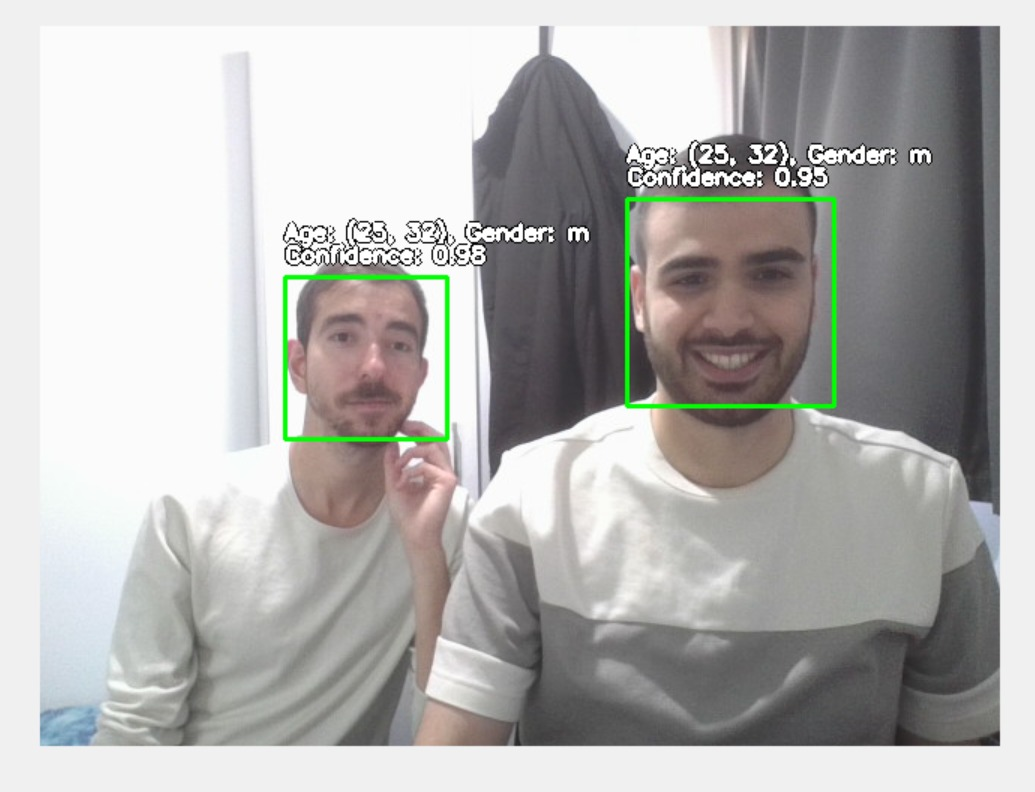
\includegraphics[width=0.8\textwidth]{assets/app.jpg}
    \caption{Real-time Age and Gender Prediction App}
    \label{fig:app}
\end{figure}

\bibliographystyle{plain}
\bibliography{references} 

\end{document}
